% Options for packages loaded elsewhere
\PassOptionsToPackage{unicode}{hyperref}
\PassOptionsToPackage{hyphens}{url}
\PassOptionsToPackage{dvipsnames,svgnames,x11names}{xcolor}
%
\documentclass[
  letterpaper,
  DIV=11,
  numbers=noendperiod]{scrartcl}

\usepackage{amsmath,amssymb}
\usepackage{iftex}
\ifPDFTeX
  \usepackage[T1]{fontenc}
  \usepackage[utf8]{inputenc}
  \usepackage{textcomp} % provide euro and other symbols
\else % if luatex or xetex
  \usepackage{unicode-math}
  \defaultfontfeatures{Scale=MatchLowercase}
  \defaultfontfeatures[\rmfamily]{Ligatures=TeX,Scale=1}
\fi
\usepackage{lmodern}
\ifPDFTeX\else  
    % xetex/luatex font selection
  \setmathfont[]{Libertinus Math}
\fi
% Use upquote if available, for straight quotes in verbatim environments
\IfFileExists{upquote.sty}{\usepackage{upquote}}{}
\IfFileExists{microtype.sty}{% use microtype if available
  \usepackage[]{microtype}
  \UseMicrotypeSet[protrusion]{basicmath} % disable protrusion for tt fonts
}{}
\makeatletter
\@ifundefined{KOMAClassName}{% if non-KOMA class
  \IfFileExists{parskip.sty}{%
    \usepackage{parskip}
  }{% else
    \setlength{\parindent}{0pt}
    \setlength{\parskip}{6pt plus 2pt minus 1pt}}
}{% if KOMA class
  \KOMAoptions{parskip=half}}
\makeatother
\usepackage{xcolor}
\usepackage[top=1in,bottom=1in,left=1in,right=1in,heightrounded]{geometry}
\setlength{\emergencystretch}{3em} % prevent overfull lines
\setcounter{secnumdepth}{-\maxdimen} % remove section numbering
% Make \paragraph and \subparagraph free-standing
\ifx\paragraph\undefined\else
  \let\oldparagraph\paragraph
  \renewcommand{\paragraph}[1]{\oldparagraph{#1}\mbox{}}
\fi
\ifx\subparagraph\undefined\else
  \let\oldsubparagraph\subparagraph
  \renewcommand{\subparagraph}[1]{\oldsubparagraph{#1}\mbox{}}
\fi

\usepackage{color}
\usepackage{fancyvrb}
\newcommand{\VerbBar}{|}
\newcommand{\VERB}{\Verb[commandchars=\\\{\}]}
\DefineVerbatimEnvironment{Highlighting}{Verbatim}{commandchars=\\\{\}}
% Add ',fontsize=\small' for more characters per line
\usepackage{framed}
\definecolor{shadecolor}{RGB}{241,243,245}
\newenvironment{Shaded}{\begin{snugshade}}{\end{snugshade}}
\newcommand{\AlertTok}[1]{\textcolor[rgb]{0.68,0.00,0.00}{#1}}
\newcommand{\AnnotationTok}[1]{\textcolor[rgb]{0.37,0.37,0.37}{#1}}
\newcommand{\AttributeTok}[1]{\textcolor[rgb]{0.40,0.45,0.13}{#1}}
\newcommand{\BaseNTok}[1]{\textcolor[rgb]{0.68,0.00,0.00}{#1}}
\newcommand{\BuiltInTok}[1]{\textcolor[rgb]{0.00,0.23,0.31}{#1}}
\newcommand{\CharTok}[1]{\textcolor[rgb]{0.13,0.47,0.30}{#1}}
\newcommand{\CommentTok}[1]{\textcolor[rgb]{0.37,0.37,0.37}{#1}}
\newcommand{\CommentVarTok}[1]{\textcolor[rgb]{0.37,0.37,0.37}{\textit{#1}}}
\newcommand{\ConstantTok}[1]{\textcolor[rgb]{0.56,0.35,0.01}{#1}}
\newcommand{\ControlFlowTok}[1]{\textcolor[rgb]{0.00,0.23,0.31}{#1}}
\newcommand{\DataTypeTok}[1]{\textcolor[rgb]{0.68,0.00,0.00}{#1}}
\newcommand{\DecValTok}[1]{\textcolor[rgb]{0.68,0.00,0.00}{#1}}
\newcommand{\DocumentationTok}[1]{\textcolor[rgb]{0.37,0.37,0.37}{\textit{#1}}}
\newcommand{\ErrorTok}[1]{\textcolor[rgb]{0.68,0.00,0.00}{#1}}
\newcommand{\ExtensionTok}[1]{\textcolor[rgb]{0.00,0.23,0.31}{#1}}
\newcommand{\FloatTok}[1]{\textcolor[rgb]{0.68,0.00,0.00}{#1}}
\newcommand{\FunctionTok}[1]{\textcolor[rgb]{0.28,0.35,0.67}{#1}}
\newcommand{\ImportTok}[1]{\textcolor[rgb]{0.00,0.46,0.62}{#1}}
\newcommand{\InformationTok}[1]{\textcolor[rgb]{0.37,0.37,0.37}{#1}}
\newcommand{\KeywordTok}[1]{\textcolor[rgb]{0.00,0.23,0.31}{#1}}
\newcommand{\NormalTok}[1]{\textcolor[rgb]{0.00,0.23,0.31}{#1}}
\newcommand{\OperatorTok}[1]{\textcolor[rgb]{0.37,0.37,0.37}{#1}}
\newcommand{\OtherTok}[1]{\textcolor[rgb]{0.00,0.23,0.31}{#1}}
\newcommand{\PreprocessorTok}[1]{\textcolor[rgb]{0.68,0.00,0.00}{#1}}
\newcommand{\RegionMarkerTok}[1]{\textcolor[rgb]{0.00,0.23,0.31}{#1}}
\newcommand{\SpecialCharTok}[1]{\textcolor[rgb]{0.37,0.37,0.37}{#1}}
\newcommand{\SpecialStringTok}[1]{\textcolor[rgb]{0.13,0.47,0.30}{#1}}
\newcommand{\StringTok}[1]{\textcolor[rgb]{0.13,0.47,0.30}{#1}}
\newcommand{\VariableTok}[1]{\textcolor[rgb]{0.07,0.07,0.07}{#1}}
\newcommand{\VerbatimStringTok}[1]{\textcolor[rgb]{0.13,0.47,0.30}{#1}}
\newcommand{\WarningTok}[1]{\textcolor[rgb]{0.37,0.37,0.37}{\textit{#1}}}

\providecommand{\tightlist}{%
  \setlength{\itemsep}{0pt}\setlength{\parskip}{0pt}}\usepackage{longtable,booktabs,array}
\usepackage{calc} % for calculating minipage widths
% Correct order of tables after \paragraph or \subparagraph
\usepackage{etoolbox}
\makeatletter
\patchcmd\longtable{\par}{\if@noskipsec\mbox{}\fi\par}{}{}
\makeatother
% Allow footnotes in longtable head/foot
\IfFileExists{footnotehyper.sty}{\usepackage{footnotehyper}}{\usepackage{footnote}}
\makesavenoteenv{longtable}
\usepackage{graphicx}
\makeatletter
\def\maxwidth{\ifdim\Gin@nat@width>\linewidth\linewidth\else\Gin@nat@width\fi}
\def\maxheight{\ifdim\Gin@nat@height>\textheight\textheight\else\Gin@nat@height\fi}
\makeatother
% Scale images if necessary, so that they will not overflow the page
% margins by default, and it is still possible to overwrite the defaults
% using explicit options in \includegraphics[width, height, ...]{}
\setkeys{Gin}{width=\maxwidth,height=\maxheight,keepaspectratio}
% Set default figure placement to htbp
\makeatletter
\def\fps@figure{htbp}
\makeatother
% definitions for citeproc citations
\NewDocumentCommand\citeproctext{}{}
\NewDocumentCommand\citeproc{mm}{%
  \begingroup\def\citeproctext{#2}\cite{#1}\endgroup}
\makeatletter
 % allow citations to break across lines
 \let\@cite@ofmt\@firstofone
 % avoid brackets around text for \cite:
 \def\@biblabel#1{}
 \def\@cite#1#2{{#1\if@tempswa , #2\fi}}
\makeatother
\newlength{\cslhangindent}
\setlength{\cslhangindent}{1.5em}
\newlength{\csllabelwidth}
\setlength{\csllabelwidth}{3em}
\newenvironment{CSLReferences}[2] % #1 hanging-indent, #2 entry-spacing
 {\begin{list}{}{%
  \setlength{\itemindent}{0pt}
  \setlength{\leftmargin}{0pt}
  \setlength{\parsep}{0pt}
  % turn on hanging indent if param 1 is 1
  \ifodd #1
   \setlength{\leftmargin}{\cslhangindent}
   \setlength{\itemindent}{-1\cslhangindent}
  \fi
  % set entry spacing
  \setlength{\itemsep}{#2\baselineskip}}}
 {\end{list}}
\usepackage{calc}
\newcommand{\CSLBlock}[1]{\hfill\break#1\hfill\break}
\newcommand{\CSLLeftMargin}[1]{\parbox[t]{\csllabelwidth}{\strut#1\strut}}
\newcommand{\CSLRightInline}[1]{\parbox[t]{\linewidth - \csllabelwidth}{\strut#1\strut}}
\newcommand{\CSLIndent}[1]{\hspace{\cslhangindent}#1}

\usepackage{booktabs}
\usepackage{longtable}
\usepackage{array}
\usepackage{multirow}
\usepackage{wrapfig}
\usepackage{float}
\usepackage{colortbl}
\usepackage{pdflscape}
\usepackage{tabu}
\usepackage{threeparttable}
\usepackage{threeparttablex}
\usepackage[normalem]{ulem}
\usepackage{makecell}
\usepackage{xcolor}
\KOMAoption{captions}{tableheading}
\makeatletter
\@ifpackageloaded{caption}{}{\usepackage{caption}}
\AtBeginDocument{%
\ifdefined\contentsname
  \renewcommand*\contentsname{Table of contents}
\else
  \newcommand\contentsname{Table of contents}
\fi
\ifdefined\listfigurename
  \renewcommand*\listfigurename{List of Figures}
\else
  \newcommand\listfigurename{List of Figures}
\fi
\ifdefined\listtablename
  \renewcommand*\listtablename{List of Tables}
\else
  \newcommand\listtablename{List of Tables}
\fi
\ifdefined\figurename
  \renewcommand*\figurename{Figure}
\else
  \newcommand\figurename{Figure}
\fi
\ifdefined\tablename
  \renewcommand*\tablename{Table}
\else
  \newcommand\tablename{Table}
\fi
}
\@ifpackageloaded{float}{}{\usepackage{float}}
\floatstyle{ruled}
\@ifundefined{c@chapter}{\newfloat{codelisting}{h}{lop}}{\newfloat{codelisting}{h}{lop}[chapter]}
\floatname{codelisting}{Listing}
\newcommand*\listoflistings{\listof{codelisting}{List of Listings}}
\makeatother
\makeatletter
\makeatother
\makeatletter
\@ifpackageloaded{caption}{}{\usepackage{caption}}
\@ifpackageloaded{subcaption}{}{\usepackage{subcaption}}
\makeatother
\ifLuaTeX
  \usepackage{selnolig}  % disable illegal ligatures
\fi
\IfFileExists{bookmark.sty}{\usepackage{bookmark}}{\usepackage{hyperref}}
\IfFileExists{xurl.sty}{\usepackage{xurl}}{} % add URL line breaks if available
\urlstyle{same} % disable monospaced font for URLs
\hypersetup{
  colorlinks=true,
  linkcolor={DarkSlateBlue},
  filecolor={Maroon},
  citecolor={DarkSlateBlue},
  urlcolor={DarkSlateBlue},
  pdfcreator={LaTeX via pandoc}}

\author{}
\date{}

\begin{document}
\begin{centering}
\LARGE
{The Role of Variability in Learning Transfer: A Similarity-Based Computational Approach}

 
\vspace*{1.5cm}

\LARGE
{Thomas E. Gorman}

\vspace{16.5cm}

\end{centering}

Submitted to the faculty of the University Graduate School in partial
fulfillment of the requirements for the degree Doctor of Philosophy in
the Department of Psychology and Brain Sciences and the Cognitive
Science Program, Indiana University Indiana University

\vspace{6cm}

\pagenumbering{gobble}

\newpage

Accepted by the Graduate Faculty, Indiana University, in partial
fulfillment of the requirements for the degree of Doctor of Philosophy.
\vspace{4cm}

\hfill\break
\_\_\_\_\_\_\_\_\_\_\_\_\_\_\_\_\_\_\_\_\_\_\_\_\_\_\_\_\_ Robert L.
Goldstone, PhD \vspace{2.5cm}\\
\strut \\
\_\_\_\_\_\_\_\_\_\_\_\_\_\_\_\_\_\_\_\_\_\_\_\_\_\_\_\_\_ Robert
Nosofsky, PhD \vspace{2.5cm}\\
\_\_\_\_\_\_\_\_\_\_\_\_\_\_\_\_\_\_\_\_\_\_\_\_\_\_\_\_\_ Peter Todd,
PhD \vspace{2.5cm}\\
\_\_\_\_\_\_\_\_\_\_\_\_\_\_\_\_\_\_\_\_\_\_\_\_\_\_\_\_\_ Mike Jones,
PhD

\newpage

\begin{centering}

\vspace*{6.5cm}

@2023 \\
\vspace{1cm} 

Thomas E. Gorman
\vspace{.2cm}

\vspace{5cm}

\end{centering}

\newpage
\begin{center}
\textbf{Acknowledgements}
\end{center}
\newpage

\newpage{}

\section{Abstract}\label{abstract}

This dissertation seeks to explore the cognitive underpinnings that
govern the generalization of learning, focusing specifically on the role
of variability during training in shaping subsequent transfer
performance. A comprehensive review of the existing literature is
presented, emphasizing the methodological complications associated with
disentangling the confounding effects of similarity. Through a series of
experiments involving several novel visuomotor tasks, this work
investigates whether and how variability in training conditions affects
performance in novel tasks. To theoretically account for the empirical
outcomes, I employ both instance-based and connectionist computational
models, both of which incorporate similarity-based mechanisms. These
models serve to account for the extent to which variability influences
the learners' generalization gradient, and also explain how training
variation can produce both beneficial and deleterious outcomes.

\newpage{}

\tableofcontents
\newpage
\listoffigures
\newpage
\listoftables
\newpage

\begin{Shaded}
\begin{Highlighting}[]
\NormalTok{pacman}\SpecialCharTok{::}\FunctionTok{p\_load}\NormalTok{(tidyr,papaja, knitr, tinytex, RColorBrewer, kableExtra, cowplot, patchwork)}
\FunctionTok{source}\NormalTok{(}\StringTok{\textquotesingle{}../Functions/IGAS\_ProcessFunctions.R\textquotesingle{}}\NormalTok{)}
\end{Highlighting}
\end{Shaded}

\[e^{(c\cdot|x-800|)}\]

\[e^{(c\cdot|x-400|)}\]

\[e^{(c\cdot|x-800|)}\] + \[e^{(c\cdot|x-400|)}\]

\[e^{(c_{varied}\cdot|x-800|)}\]

\(e^{(c_{varied}\cdot|x-800|)}\) \(+e^{(c_{varied}\cdot|x-400|)}\)
\(e^{(c_{varied}\cdot|x-800|)}+e^{(c_{varied}\cdot|x-400|)}\)

\(e^{(c\cdot|x-800|)} + e^{(c\cdot|x-400|)}\),

\begin{Shaded}
\begin{Highlighting}[]
\CommentTok{\# }

\NormalTok{p}\OtherTok{=}\DecValTok{2}
\NormalTok{c}\OtherTok{\textless{}{-}}\NormalTok{ .}\DecValTok{000002}

\NormalTok{trainingTestingDifference}\OtherTok{=}\DecValTok{2000}\NormalTok{;}
\NormalTok{cvaried}\OtherTok{=}\NormalTok{.}\DecValTok{00002}
\NormalTok{cconstant}\OtherTok{=}\NormalTok{.}\DecValTok{0005}
\NormalTok{simdat }\OtherTok{\textless{}{-}} \FunctionTok{data.frame}\NormalTok{(}\AttributeTok{x=}\FunctionTok{rep}\NormalTok{(}\FunctionTok{seq}\NormalTok{(}\DecValTok{200}\NormalTok{,}\DecValTok{1000}\NormalTok{),}\DecValTok{3}\NormalTok{),}\AttributeTok{condit=}\FunctionTok{c}\NormalTok{(}\FunctionTok{rep}\NormalTok{(}\StringTok{"varied"}\NormalTok{,}\DecValTok{1602}\NormalTok{),}\FunctionTok{rep}\NormalTok{(}\StringTok{"constant"}\NormalTok{,}\DecValTok{801}\NormalTok{)),}
                     \AttributeTok{train.position=}\FunctionTok{c}\NormalTok{(}\FunctionTok{rep}\NormalTok{(}\DecValTok{400}\NormalTok{,}\DecValTok{801}\NormalTok{),}\FunctionTok{rep}\NormalTok{(}\DecValTok{800}\NormalTok{,}\DecValTok{801}\NormalTok{),}\FunctionTok{rep}\NormalTok{(}\DecValTok{600}\NormalTok{,}\DecValTok{801}\NormalTok{)),}\AttributeTok{c=}\NormalTok{.}\DecValTok{0002}\NormalTok{,}\AttributeTok{p=}\DecValTok{2}\NormalTok{) }\SpecialCharTok{\%\textgreater{}\%}
                     \FunctionTok{mutate}\NormalTok{(}\AttributeTok{c2=}\FunctionTok{ifelse}\NormalTok{(condit}\SpecialCharTok{==}\StringTok{"varied"}\NormalTok{,cvaried,cconstant),}
                            \AttributeTok{genGauss=}\FunctionTok{exp}\NormalTok{(}\SpecialCharTok{{-}}\NormalTok{c}\SpecialCharTok{*}\NormalTok{(}\FunctionTok{abs}\NormalTok{((x}\SpecialCharTok{{-}}\NormalTok{train.position)}\SpecialCharTok{\^{}}\NormalTok{p))),}
                            \AttributeTok{genGaussDist=}\FunctionTok{exp}\NormalTok{(}\SpecialCharTok{{-}}\NormalTok{c}\SpecialCharTok{*}\NormalTok{(trainingTestingDifference}\SpecialCharTok{+}\FunctionTok{abs}\NormalTok{((x}\SpecialCharTok{{-}}\NormalTok{train.position)}\SpecialCharTok{\^{}}\NormalTok{p))),}
                            \AttributeTok{genGauss2=}\FunctionTok{exp}\NormalTok{(}\SpecialCharTok{{-}}\NormalTok{c2}\SpecialCharTok{*}\NormalTok{(}\FunctionTok{abs}\NormalTok{((x}\SpecialCharTok{{-}}\NormalTok{train.position)}\SpecialCharTok{\^{}}\NormalTok{p))),}
                            \AttributeTok{genGaussDist2=}\FunctionTok{exp}\NormalTok{(}\SpecialCharTok{{-}}\NormalTok{c2}\SpecialCharTok{*}\NormalTok{(trainingTestingDifference}\SpecialCharTok{+}\FunctionTok{abs}\NormalTok{((x}\SpecialCharTok{{-}}\NormalTok{train.position)}\SpecialCharTok{\^{}}\NormalTok{p))),}
\NormalTok{                            ) }\SpecialCharTok{\%\textgreater{}\%} 
  \FunctionTok{group\_by}\NormalTok{(x,condit) }\SpecialCharTok{\%\textgreater{}\%}
  \FunctionTok{summarise}\NormalTok{(}\AttributeTok{genGauss=}\FunctionTok{mean}\NormalTok{(genGauss),}\AttributeTok{genGauss2=}\FunctionTok{mean}\NormalTok{(genGauss2),}\AttributeTok{genGaussDist=}\FunctionTok{mean}\NormalTok{(genGaussDist),}\AttributeTok{genGaussDist2=}\FunctionTok{mean}\NormalTok{(genGaussDist2),}\AttributeTok{.groups=}\StringTok{\textquotesingle{}keep\textquotesingle{}}\NormalTok{)}


\CommentTok{\#plot(x,exp(c*(trainingTestingDifference+abs(x{-}800)))+exp(c*(trainingTestingDifference+abs(x{-}400)))}

\NormalTok{colorVec}\OtherTok{=}\FunctionTok{c}\NormalTok{(}\StringTok{"darkblue"}\NormalTok{,}\StringTok{"darkred"}\NormalTok{)}
\NormalTok{plotSpecs }\OtherTok{\textless{}{-}} \FunctionTok{list}\NormalTok{(}\FunctionTok{geom\_line}\NormalTok{(}\AttributeTok{alpha=}\NormalTok{.}\DecValTok{7}\NormalTok{),}\FunctionTok{scale\_color\_manual}\NormalTok{(}\AttributeTok{values=}\NormalTok{colorVec),}
                  \FunctionTok{geom\_vline}\NormalTok{(}\AttributeTok{alpha=}\NormalTok{.}\DecValTok{55}\NormalTok{,}\AttributeTok{xintercept =} \FunctionTok{c}\NormalTok{(}\DecValTok{400}\NormalTok{,}\DecValTok{800}\NormalTok{),}\AttributeTok{color=}\NormalTok{colorVec[}\DecValTok{2}\NormalTok{]),}
                  \FunctionTok{geom\_vline}\NormalTok{(}\AttributeTok{alpha=}\NormalTok{.}\DecValTok{55}\NormalTok{,}\AttributeTok{xintercept =} \FunctionTok{c}\NormalTok{(}\DecValTok{600}\NormalTok{),}\AttributeTok{color=}\NormalTok{colorVec[}\DecValTok{1}\NormalTok{]),}
                  \FunctionTok{ylim}\NormalTok{(}\FunctionTok{c}\NormalTok{(}\DecValTok{0}\NormalTok{,}\FloatTok{1.05}\NormalTok{)),}
                  \CommentTok{\#xlim(c(250,950)),}
                  \FunctionTok{scale\_x\_continuous}\NormalTok{(}\AttributeTok{breaks=}\FunctionTok{seq}\NormalTok{(}\DecValTok{200}\NormalTok{,}\DecValTok{1000}\NormalTok{,}\AttributeTok{by=}\DecValTok{200}\NormalTok{)),}
                  \FunctionTok{xlab}\NormalTok{(}\StringTok{"Test Stimulus"}\NormalTok{),}
                  \FunctionTok{annotate}\NormalTok{(}\AttributeTok{geom=}\StringTok{"text"}\NormalTok{,}\AttributeTok{x=}\DecValTok{455}\NormalTok{,}\AttributeTok{y=}\FloatTok{1.05}\NormalTok{,}\AttributeTok{label=}\StringTok{"Varied"}\NormalTok{,}\AttributeTok{size=}\FloatTok{3.0}\NormalTok{),}
                  \FunctionTok{annotate}\NormalTok{(}\AttributeTok{geom=}\StringTok{"text"}\NormalTok{,}\AttributeTok{x=}\DecValTok{455}\NormalTok{,}\AttributeTok{y=}\NormalTok{.}\DecValTok{97}\NormalTok{,}\AttributeTok{label=}\StringTok{"Training"}\NormalTok{,}\AttributeTok{size=}\FloatTok{3.0}\NormalTok{),}
                  \FunctionTok{annotate}\NormalTok{(}\AttributeTok{geom=}\StringTok{"text"}\NormalTok{,}\AttributeTok{x=}\DecValTok{662}\NormalTok{,}\AttributeTok{y=}\FloatTok{1.05}\NormalTok{,}\AttributeTok{label=}\StringTok{"Constant"}\NormalTok{,}\AttributeTok{size=}\FloatTok{3.0}\NormalTok{),}
                  \FunctionTok{annotate}\NormalTok{(}\AttributeTok{geom=}\StringTok{"text"}\NormalTok{,}\AttributeTok{x=}\DecValTok{657}\NormalTok{,}\AttributeTok{y=}\NormalTok{.}\DecValTok{97}\NormalTok{,}\AttributeTok{label=}\StringTok{"Training"}\NormalTok{,}\AttributeTok{size=}\FloatTok{3.0}\NormalTok{),}
                  \FunctionTok{annotate}\NormalTok{(}\AttributeTok{geom=}\StringTok{"text"}\NormalTok{,}\AttributeTok{x=}\DecValTok{855}\NormalTok{,}\AttributeTok{y=}\FloatTok{1.05}\NormalTok{,}\AttributeTok{label=}\StringTok{"Varied"}\NormalTok{,}\AttributeTok{size=}\FloatTok{3.0}\NormalTok{),}
                  \FunctionTok{annotate}\NormalTok{(}\AttributeTok{geom=}\StringTok{"text"}\NormalTok{,}\AttributeTok{x=}\DecValTok{855}\NormalTok{,}\AttributeTok{y=}\NormalTok{.}\DecValTok{97}\NormalTok{,}\AttributeTok{label=}\StringTok{"Training"}\NormalTok{,}\AttributeTok{size=}\FloatTok{3.0}\NormalTok{),}
                  \FunctionTok{theme}\NormalTok{(}\AttributeTok{panel.border =} \FunctionTok{element\_rect}\NormalTok{(}\AttributeTok{colour =} \StringTok{"black"}\NormalTok{, }\AttributeTok{fill=}\ConstantTok{NA}\NormalTok{, }\AttributeTok{size=}\DecValTok{1}\NormalTok{),}
                        \AttributeTok{legend.position=}\StringTok{"none"}\NormalTok{))}

\NormalTok{ip1 }\OtherTok{\textless{}{-}}\NormalTok{ simdat  }\SpecialCharTok{\%\textgreater{}\%} \FunctionTok{ggplot}\NormalTok{(}\FunctionTok{aes}\NormalTok{(x,}\AttributeTok{y=}\NormalTok{genGauss,}\AttributeTok{group=}\NormalTok{condit,}\AttributeTok{col=}\NormalTok{condit))}\SpecialCharTok{+}\NormalTok{plotSpecs}\SpecialCharTok{+}\FunctionTok{ylab}\NormalTok{(}\StringTok{"Amount of Generalization"}\NormalTok{)}\SpecialCharTok{+}\FunctionTok{ggtitle}\NormalTok{(}\StringTok{"Identical context, 1c"}\NormalTok{)}
\NormalTok{ip2 }\OtherTok{\textless{}{-}}\NormalTok{ simdat }\SpecialCharTok{\%\textgreater{}\%}  \FunctionTok{ggplot}\NormalTok{(}\FunctionTok{aes}\NormalTok{(x,}\AttributeTok{y=}\NormalTok{genGauss2,}\AttributeTok{group=}\NormalTok{condit,}\AttributeTok{col=}\NormalTok{condit))}\SpecialCharTok{+}\NormalTok{plotSpecs}\SpecialCharTok{+}\FunctionTok{ylab}\NormalTok{(}\StringTok{""}\NormalTok{)}\SpecialCharTok{+}\FunctionTok{ggtitle}\NormalTok{(}\StringTok{"Identical context, 2c"}\NormalTok{)}
\NormalTok{ip3 }\OtherTok{\textless{}{-}}\NormalTok{ simdat  }\SpecialCharTok{\%\textgreater{}\%} \FunctionTok{ggplot}\NormalTok{(}\FunctionTok{aes}\NormalTok{(x,}\AttributeTok{y=}\NormalTok{genGaussDist,}\AttributeTok{group=}\NormalTok{condit,}\AttributeTok{col=}\NormalTok{condit))}\SpecialCharTok{+}\NormalTok{plotSpecs}\SpecialCharTok{+}\FunctionTok{ylab}\NormalTok{(}\StringTok{"Amount of Generalization"}\NormalTok{)}\SpecialCharTok{+}
  \FunctionTok{ggtitle}\NormalTok{(}\StringTok{"Added distance due to context, 1c"}\NormalTok{)}\SpecialCharTok{+}\FunctionTok{theme}\NormalTok{(}\AttributeTok{plot.margin =} \FunctionTok{margin}\NormalTok{(}\DecValTok{0}\NormalTok{, }\DecValTok{0}\NormalTok{, }\DecValTok{0}\NormalTok{, }\DecValTok{1}\NormalTok{))}
\NormalTok{ip4 }\OtherTok{\textless{}{-}}\NormalTok{ simdat }\SpecialCharTok{\%\textgreater{}\%}  \FunctionTok{ggplot}\NormalTok{(}\FunctionTok{aes}\NormalTok{(x,}\AttributeTok{y=}\NormalTok{genGaussDist2,}\AttributeTok{group=}\NormalTok{condit,}\AttributeTok{col=}\NormalTok{condit))}\SpecialCharTok{+}\NormalTok{plotSpecs}\SpecialCharTok{+}\FunctionTok{ylab}\NormalTok{(}\StringTok{""}\NormalTok{)}\SpecialCharTok{+}
  \FunctionTok{ggtitle}\NormalTok{(}\StringTok{"Added distance due to context, 2c"}\NormalTok{)}\SpecialCharTok{+}\FunctionTok{theme}\NormalTok{(}\AttributeTok{plot.margin =} \FunctionTok{margin}\NormalTok{(}\DecValTok{0}\NormalTok{, }\DecValTok{0}\NormalTok{, }\DecValTok{0}\NormalTok{, }\DecValTok{1}\NormalTok{))}
\CommentTok{\# gridExtra::grid.arrange(ip1,ip2,ip3,ip4,ncol=2)}

\NormalTok{gtitle}\OtherTok{=}\StringTok{"Figure 9."}
\NormalTok{title }\OtherTok{=} \FunctionTok{ggdraw}\NormalTok{()}\SpecialCharTok{+}\FunctionTok{draw\_label}\NormalTok{(gtitle,}\AttributeTok{fontface =} \StringTok{\textquotesingle{}bold\textquotesingle{}}\NormalTok{,}\AttributeTok{x=}\DecValTok{0}\NormalTok{,}\AttributeTok{hjust=}\DecValTok{0}\NormalTok{,}\AttributeTok{size=}\DecValTok{11}\NormalTok{)}\SpecialCharTok{+}\FunctionTok{theme}\NormalTok{(}\AttributeTok{plot.margin =} \FunctionTok{margin}\NormalTok{(}\DecValTok{0}\NormalTok{, }\DecValTok{0}\NormalTok{, }\DecValTok{0}\NormalTok{, }\DecValTok{1}\NormalTok{))}
\FunctionTok{plot\_grid}\NormalTok{(title,}\ConstantTok{NULL}\NormalTok{,ip1,ip2,ip3,ip4,}\AttributeTok{ncol=}\DecValTok{2}\NormalTok{,}\AttributeTok{rel\_heights=}\FunctionTok{c}\NormalTok{(.}\DecValTok{1}\NormalTok{,.}\DecValTok{8}\NormalTok{,.}\DecValTok{8}\NormalTok{))}
\end{Highlighting}
\end{Shaded}

\begin{figure}[H]

\centering{

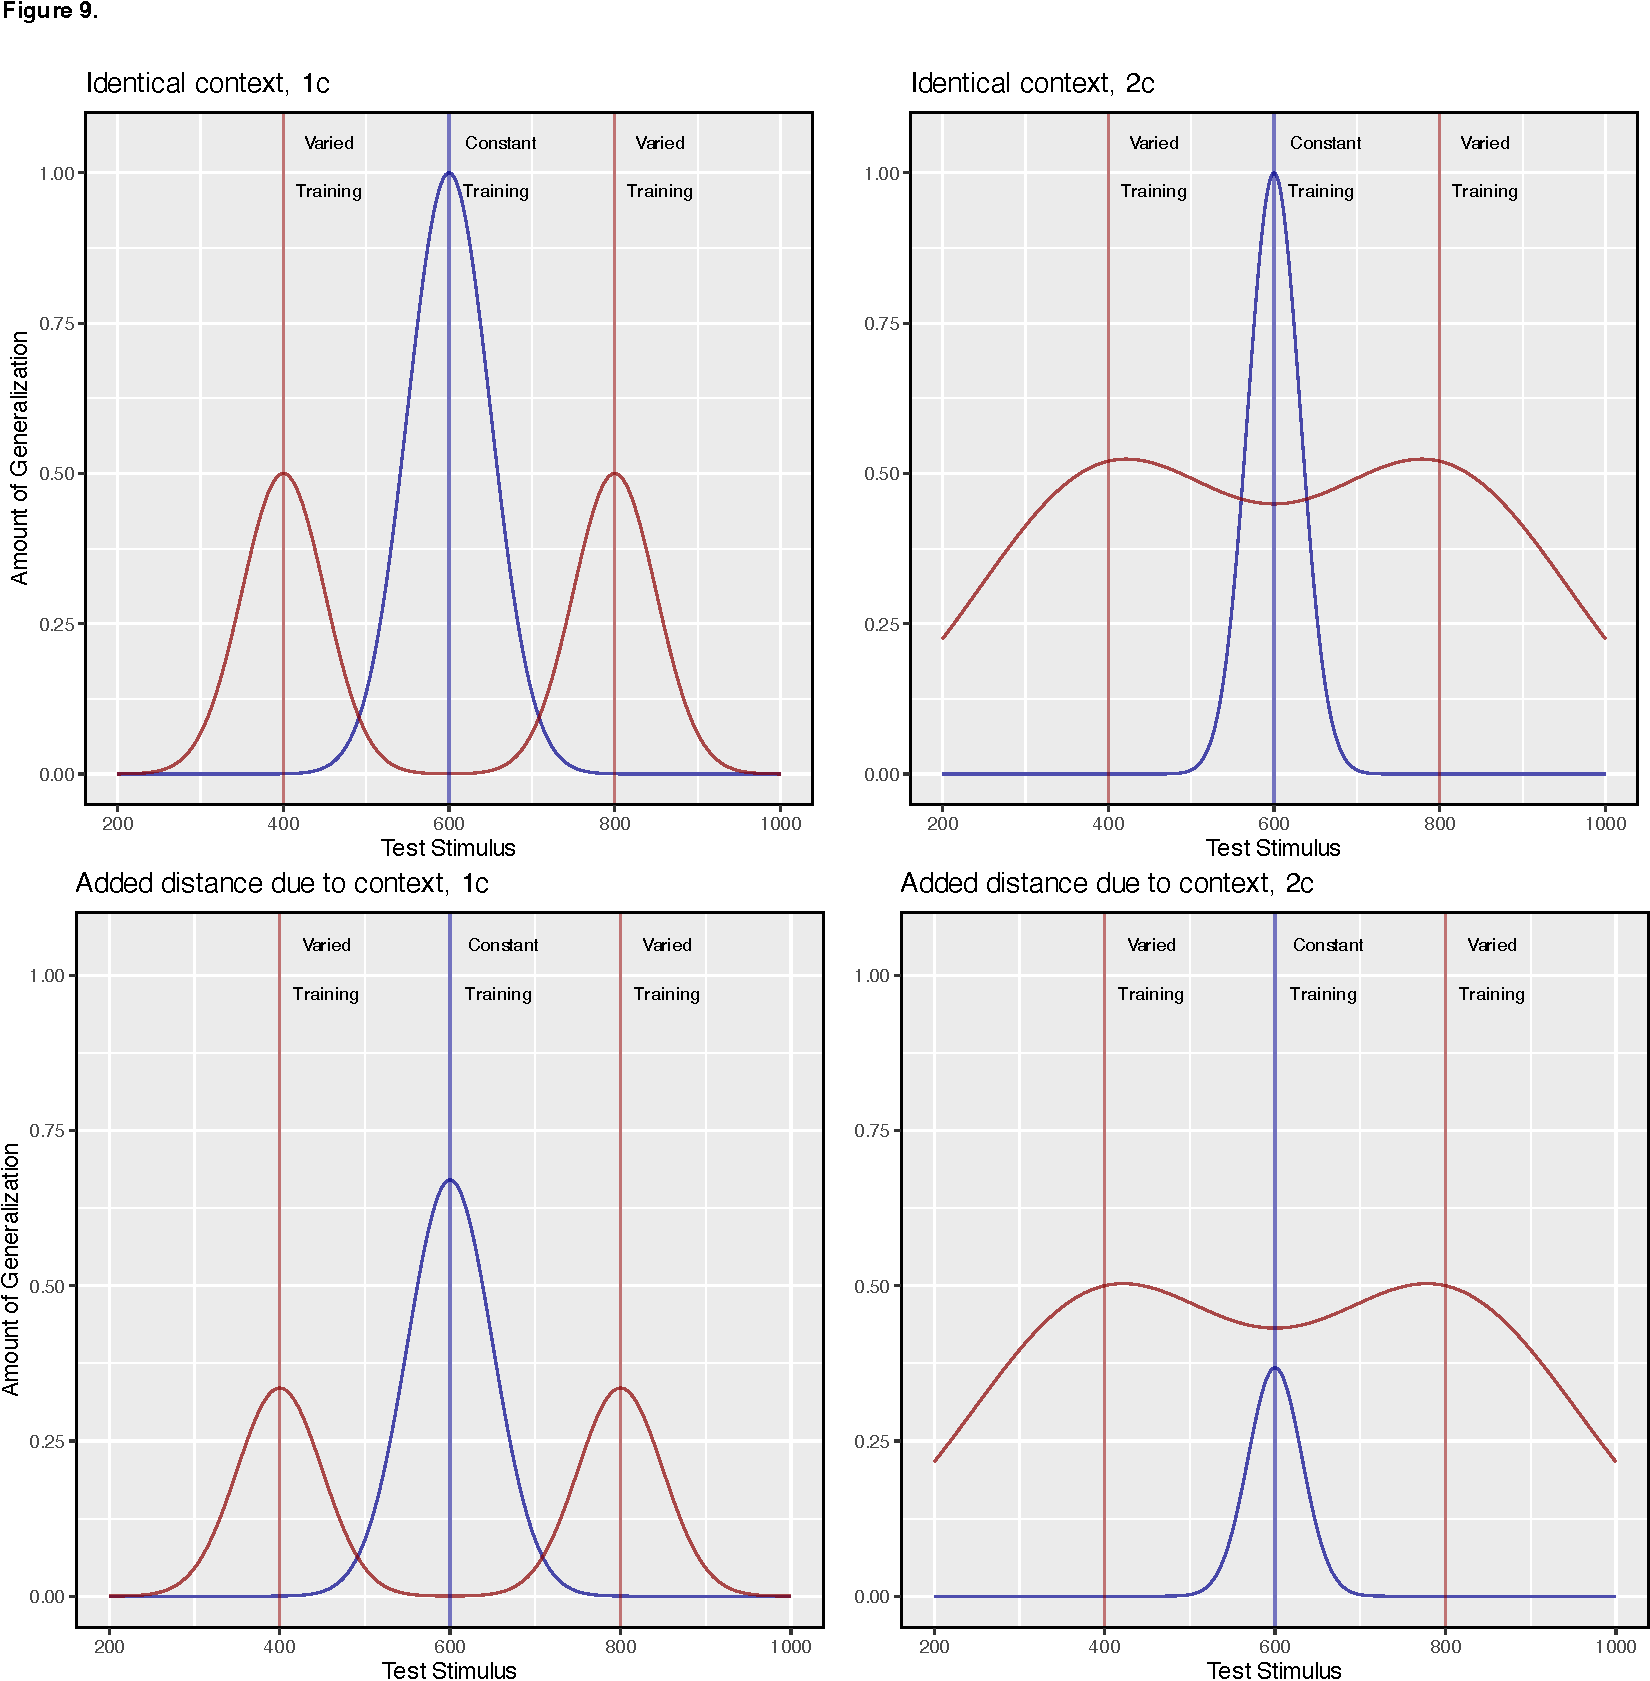
\includegraphics{igas_e1_files/figure-pdf/fig-Toy-Model2-1.pdf}

}

\caption{\label{fig-Toy-Model2}A simple model depicting the necessity of
both of two separately fit generalization parameters, c, and a positive
distance between training and testing contexts, in order for an instance
model to predict a pattern of varied training from stimuli 400 and 800
outperforming constant training from position 600 at a test position of
600. For the top left panel, in which the generalization model assumes a
single c value (-.008) for both varied and constant conditions, and
identical contexts across training and testing, the equation which
generates the varied condition is - Amount of Generalization =
\(e^{(c\cdot|x-800|)} + e^{(c\cdot|x-400|)}\), whereas the constant
group generalization is generated from \(2\cdot e^{(c\cdot|x-600|)}\).
For the top right panel, the c constants in the original equations are
different for the 2 conditions, with \(c=-.002\) for the varied
condition, and \(c=-.008\) for the constant condition. The bottom two
panels are generated from identical equations to those immediately
above, except for the addition of extra distance (100 units) to reflect
the assumption of some change in context between training and testing
conditions. Thus, the generalization model for the varied condition in
the bottom-right panel is of the form - Amount of Generalization =
\(e^{(c_{varied}\cdot|x-800|)}+e^{(c_{varied}\cdot|x-400|)}\) .}

\end{figure}%

\newpage{}

\subsection{Main body}\label{main-body}

Following the procedure used by Mcdaniel et al.
(\citeproc{ref-mcdanielPredictingTransferPerformance2009}{2009}), we
will assess the ability of both ALM and EXAM to account for the
empirical data when fitting the models to 1) only the training data, and
2) both training and testing data. Models will be fit directly to the
trial by trial data of each individual participants, both by minimizing
the root-mean squared deviation (RMSE), and by maximizing log
likelihood. Because ALM has been shown to do poorly at accounting for
human patterns extrapolation
(\citeproc{ref-deloshExtrapolationSineQua1997}{DeLosh et al., 1997}), we
will also fit the extended EXAM version of the model, which operates
identically to ALM during training, but includes a linear extrapolation
mechanism for generating novel responses during testing.

quarto pandoc --citeproc --pdf-engine xelatex -t pdf\\
--bibliography=../Assets/Bib/Dissertation.bib\\
--standalone\\
-f markdown igas\_e1.pdf.md\\
-o refer-test.pdf

quarto render igas\_e1.qmd --citeproc --pdf-engine xelatex -t pdf\\
--bibliography=../Assets/Bib/Dissertation.bib\\
--standalone\\
-o refer-test.pdf

\section{Appendix}\label{appendix}

\begin{Shaded}
\begin{Highlighting}[]
\CommentTok{\# print(getwd())}
\CommentTok{\# here::set\_here(path=\textquotesingle{}..\textquotesingle{})}
\CommentTok{\# print(getwd())}
\FunctionTok{source}\NormalTok{(here}\SpecialCharTok{::}\FunctionTok{here}\NormalTok{(}\StringTok{"Functions"}\NormalTok{, }\StringTok{"packages.R"}\NormalTok{))}
\end{Highlighting}
\end{Shaded}

\begin{Shaded}
\begin{Highlighting}[]
\NormalTok{test }\OtherTok{\textless{}{-}} \FunctionTok{readRDS}\NormalTok{(here}\SpecialCharTok{::}\FunctionTok{here}\NormalTok{(}\StringTok{"data/e1\_08{-}21{-}23.rds"}\NormalTok{)) }\SpecialCharTok{|\textgreater{}} \FunctionTok{filter}\NormalTok{(expMode2 }\SpecialCharTok{==} \StringTok{"Test"}\NormalTok{)  }\SpecialCharTok{|\textgreater{}}
  \FunctionTok{select}\NormalTok{(id,condit,bandInt,vb,vx,dist,sdist,bandType,tOrder)}
\end{Highlighting}
\end{Shaded}

\paragraph{Posterior Predictive
Distributions}\label{posterior-predictive-distributions}

\begin{Shaded}
\begin{Highlighting}[]
\NormalTok{dist\_pred }\OtherTok{\textless{}{-}} 
  \FunctionTok{posterior\_predict}\NormalTok{(e1\_distBMM, }\AttributeTok{ndraws =} \DecValTok{500}\NormalTok{) }\SpecialCharTok{|\textgreater{}} 
  \FunctionTok{array\_branch}\NormalTok{(}\AttributeTok{margin=}\DecValTok{1}\NormalTok{) }\SpecialCharTok{|\textgreater{}} 
   \FunctionTok{map\_dfr}\NormalTok{( }
    \ControlFlowTok{function}\NormalTok{(yrep\_iter) \{}
\NormalTok{      test  }\SpecialCharTok{|\textgreater{}}
        \FunctionTok{mutate}\NormalTok{(}\AttributeTok{dist\_pred =}\NormalTok{ yrep\_iter)}
\NormalTok{    \},}
    \AttributeTok{.id =} \StringTok{\textquotesingle{}iter\textquotesingle{}}
\NormalTok{  ) }\SpecialCharTok{|\textgreater{}}
  \FunctionTok{mutate}\NormalTok{(}\AttributeTok{iter =} \FunctionTok{as.numeric}\NormalTok{(iter))}



\NormalTok{dist\_pred  }\SpecialCharTok{|\textgreater{}}
  \FunctionTok{filter}\NormalTok{(iter }\SpecialCharTok{\textless{}} \DecValTok{100}\NormalTok{) }\SpecialCharTok{\%\textgreater{}\%}
  \FunctionTok{ggplot}\NormalTok{(}\FunctionTok{aes}\NormalTok{(dist\_pred, }\AttributeTok{group =}\NormalTok{ iter)) }\SpecialCharTok{+}
  \FunctionTok{geom\_line}\NormalTok{(}\AttributeTok{alpha =}\NormalTok{ .}\DecValTok{03}\NormalTok{, }\AttributeTok{stat =} \StringTok{\textquotesingle{}density\textquotesingle{}}\NormalTok{, }\AttributeTok{color =} \StringTok{\textquotesingle{}blue\textquotesingle{}}\NormalTok{) }\SpecialCharTok{+}
  \FunctionTok{geom\_density}\NormalTok{(}\AttributeTok{data =}\NormalTok{ test,}
               \FunctionTok{aes}\NormalTok{(dist,}\AttributeTok{col=}\NormalTok{vb),}
               \AttributeTok{inherit.aes =} \ConstantTok{FALSE}\NormalTok{,}
               \AttributeTok{size =} \FloatTok{0.7}\NormalTok{) }\SpecialCharTok{+} \CommentTok{\# 1}
  \FunctionTok{facet\_grid}\NormalTok{(condit }\SpecialCharTok{\textasciitilde{}}\NormalTok{ vb) }\SpecialCharTok{+}
  \FunctionTok{xlab}\NormalTok{(}\StringTok{\textquotesingle{}Deviation\textquotesingle{}}\NormalTok{)}
\end{Highlighting}
\end{Shaded}

\begin{figure}[H]

\centering{

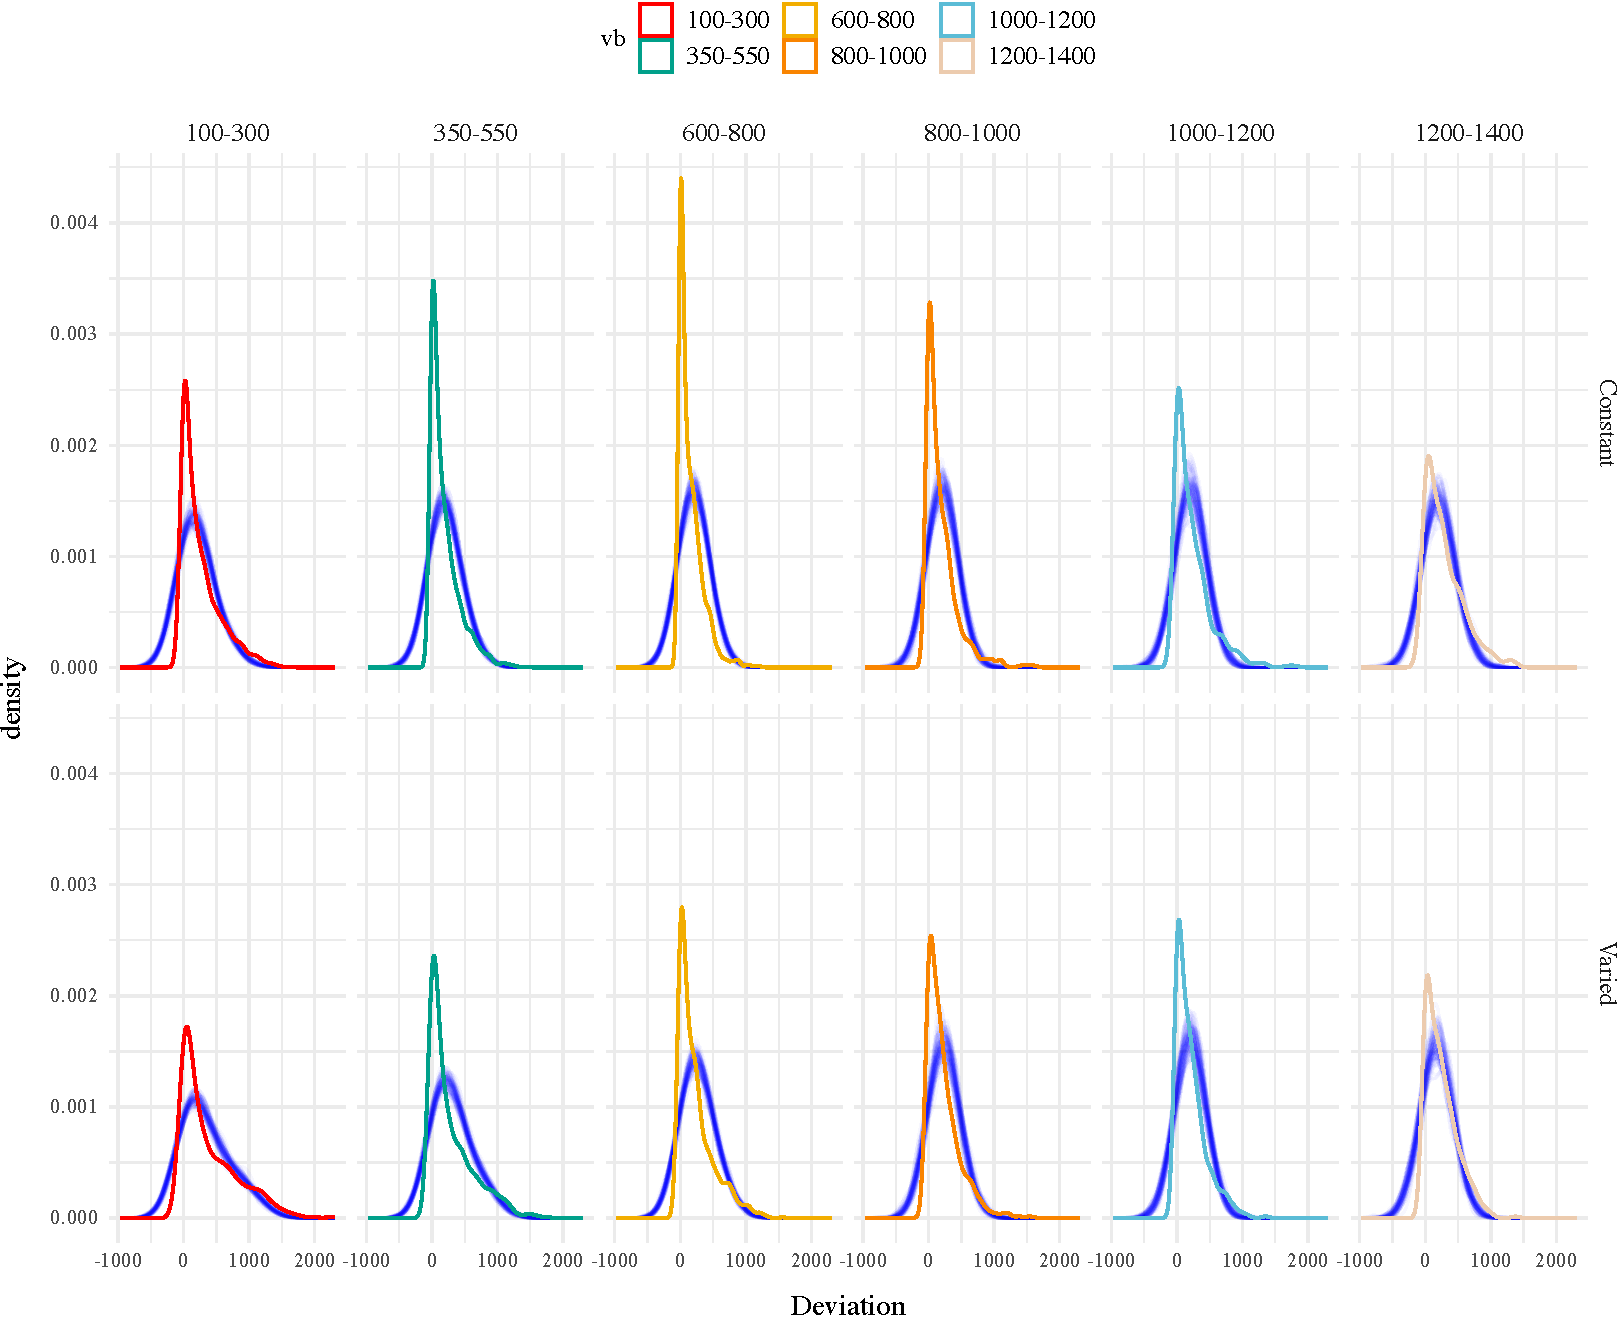
\includegraphics{igas_e1_files/figure-pdf/fig-post-pred-dist-1.pdf}

}

\caption{\label{fig-post-pred-dist}Posterior Predictive distributions
for Absolute Deviance. Posterior Draws in Blue, colored lines are
empirical data.}

\end{figure}%

\begin{Shaded}
\begin{Highlighting}[]
\NormalTok{vx\_pred }\OtherTok{\textless{}{-}} 
  \FunctionTok{posterior\_predict}\NormalTok{(e1\_vxBMM, }\AttributeTok{ndraws =} \DecValTok{500}\NormalTok{) }\SpecialCharTok{|\textgreater{}} 
  \FunctionTok{array\_branch}\NormalTok{(}\AttributeTok{margin=}\DecValTok{1}\NormalTok{) }\SpecialCharTok{|\textgreater{}} 
   \FunctionTok{map\_dfr}\NormalTok{( }
    \ControlFlowTok{function}\NormalTok{(yrep\_iter) \{}
\NormalTok{      test  }\SpecialCharTok{|\textgreater{}}
        \FunctionTok{mutate}\NormalTok{(}\AttributeTok{vx\_pred =}\NormalTok{ yrep\_iter)}
\NormalTok{    \},}
    \AttributeTok{.id =} \StringTok{\textquotesingle{}iter\textquotesingle{}}
\NormalTok{  ) }\SpecialCharTok{|\textgreater{}}
  \FunctionTok{mutate}\NormalTok{(}\AttributeTok{iter =} \FunctionTok{as.numeric}\NormalTok{(iter))}



\NormalTok{vx\_pred  }\SpecialCharTok{|\textgreater{}}
  \FunctionTok{filter}\NormalTok{(iter }\SpecialCharTok{\textless{}} \DecValTok{100}\NormalTok{) }\SpecialCharTok{\%\textgreater{}\%}
  \FunctionTok{ggplot}\NormalTok{(}\FunctionTok{aes}\NormalTok{(vx\_pred, }\AttributeTok{group =}\NormalTok{ iter)) }\SpecialCharTok{+}
  \FunctionTok{geom\_line}\NormalTok{(}\AttributeTok{alpha =}\NormalTok{ .}\DecValTok{03}\NormalTok{, }\AttributeTok{stat =} \StringTok{\textquotesingle{}density\textquotesingle{}}\NormalTok{, }\AttributeTok{color =} \StringTok{\textquotesingle{}blue\textquotesingle{}}\NormalTok{) }\SpecialCharTok{+}
  \FunctionTok{geom\_density}\NormalTok{(}\AttributeTok{data =}\NormalTok{ test,}
               \FunctionTok{aes}\NormalTok{(vx,}\AttributeTok{col=}\NormalTok{vb),}
               \AttributeTok{inherit.aes =} \ConstantTok{FALSE}\NormalTok{,}
               \AttributeTok{size =} \FloatTok{0.7}\NormalTok{) }\SpecialCharTok{+} \CommentTok{\# 1}
  \FunctionTok{facet\_grid}\NormalTok{(condit }\SpecialCharTok{\textasciitilde{}}\NormalTok{ vb) }\SpecialCharTok{+}
  \FunctionTok{xlab}\NormalTok{(}\StringTok{\textquotesingle{}Vx\textquotesingle{}}\NormalTok{)}
\end{Highlighting}
\end{Shaded}

\begin{figure}[H]

\centering{

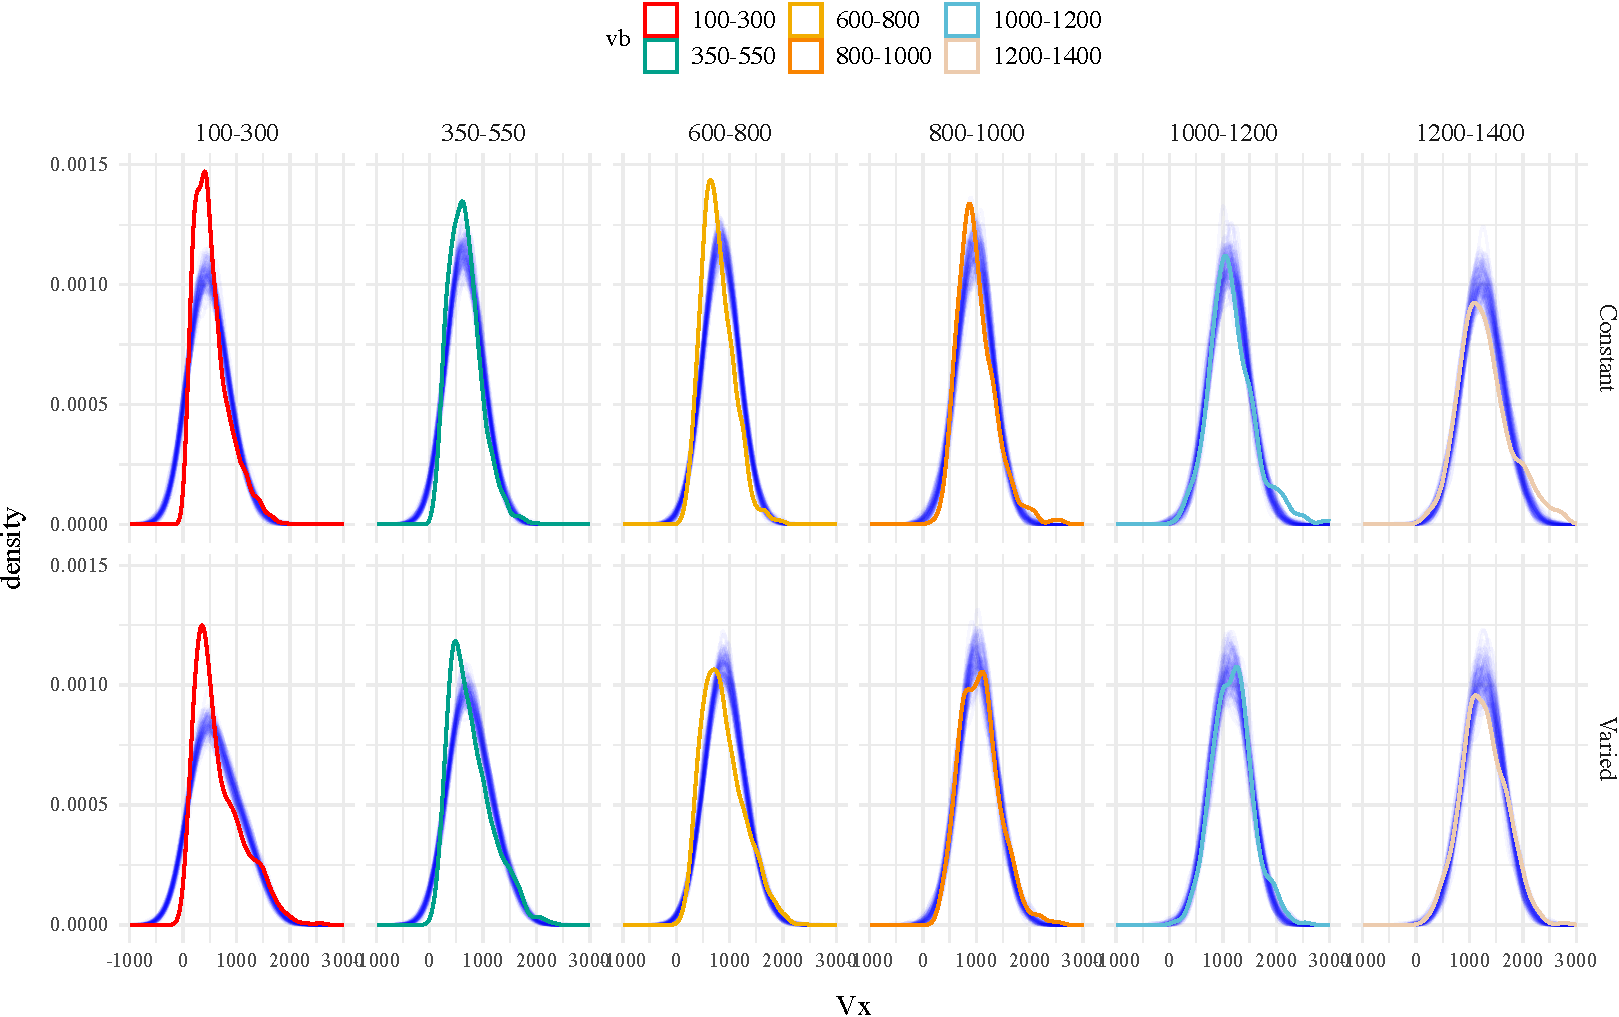
\includegraphics{igas_e1_files/figure-pdf/fig-post-pred-vx-1.pdf}

}

\caption{\label{fig-post-pred-vx}Posterior Predictive distributions for
Vx. Posterior Draws in Blue, colored lines are empirical data.}

\end{figure}%

\paragraph{Empirical vs.~Predicted}\label{empirical-vs.-predicted}

\begin{Shaded}
\begin{Highlighting}[]
\NormalTok{\{}
\NormalTok{vx\_pred  }\SpecialCharTok{|\textgreater{}}
  \FunctionTok{filter}\NormalTok{(iter }\SpecialCharTok{\textless{}} \DecValTok{100}\NormalTok{)  }\SpecialCharTok{|\textgreater{}} \FunctionTok{group\_by}\NormalTok{(id,condit,vb,iter) }\SpecialCharTok{|\textgreater{}}
  \FunctionTok{summarise}\NormalTok{(}\AttributeTok{vx\_pred=}\FunctionTok{mean}\NormalTok{(vx\_pred)) }\SpecialCharTok{\%\textgreater{}\%}
  \FunctionTok{ggplot}\NormalTok{(}\FunctionTok{aes}\NormalTok{(}\AttributeTok{x=}\NormalTok{vb,}\AttributeTok{y=}\NormalTok{vx\_pred,}\AttributeTok{fill=}\NormalTok{condit)) }\SpecialCharTok{+} 
  \FunctionTok{geom\_flat\_violin}\NormalTok{( }\AttributeTok{position =} \FunctionTok{position\_nudge}\NormalTok{(}\AttributeTok{x =} \FloatTok{0.1}\NormalTok{, }\AttributeTok{y =} \DecValTok{0}\NormalTok{),}
                   \AttributeTok{adjust =} \FloatTok{1.5}\NormalTok{,}
                   \AttributeTok{trim =} \ConstantTok{FALSE}\NormalTok{, }\AttributeTok{alpha =}\NormalTok{ .}\DecValTok{5}\NormalTok{, }\AttributeTok{colour =} \ConstantTok{NA}\NormalTok{) }\SpecialCharTok{+}
  \CommentTok{\# geom\_point(aes(x = as.numeric(vb) {-} 0.15, y = vx\_pred, colour = vb),}
  \CommentTok{\#            position = position\_jitter(width = 0.05, height = 0),}
  \CommentTok{\#            size = 1, shape = 20) +}
  \FunctionTok{geom\_boxplot}\NormalTok{(}\FunctionTok{aes}\NormalTok{(}\AttributeTok{x =}\NormalTok{ vb, }\AttributeTok{y =}\NormalTok{ vx\_pred, }\AttributeTok{fill =}\NormalTok{ condit),}
               \AttributeTok{outlier.shape =} \ConstantTok{NA}\NormalTok{,}
               \AttributeTok{alpha =} \FloatTok{0.5}\NormalTok{,}
               \AttributeTok{width =} \FloatTok{0.1}\NormalTok{,}
               \AttributeTok{colour =} \StringTok{"black"}\NormalTok{) }\SpecialCharTok{+}
  \FunctionTok{geom\_hline}\NormalTok{(}\AttributeTok{yintercept =} \DecValTok{0}\NormalTok{,}
             \AttributeTok{linetype =} \StringTok{\textquotesingle{}dashed\textquotesingle{}}\NormalTok{,}
             \AttributeTok{color =} \StringTok{\textquotesingle{}red\textquotesingle{}}\NormalTok{,}
             \AttributeTok{size =} \FloatTok{0.4}\NormalTok{) }\SpecialCharTok{+} 
  \FunctionTok{coord\_flip}\NormalTok{() }\SpecialCharTok{+} \FunctionTok{ggtitle}\NormalTok{(}\StringTok{"Predicted Vx"}\NormalTok{)  }
\NormalTok{\} }\SpecialCharTok{/}\NormalTok{ \{}
\NormalTok{vx\_pred  }\SpecialCharTok{|\textgreater{}}
  \FunctionTok{filter}\NormalTok{(iter }\SpecialCharTok{\textless{}} \DecValTok{2}\NormalTok{)  }\SpecialCharTok{|\textgreater{}} \FunctionTok{group\_by}\NormalTok{(id,condit,vb) }\SpecialCharTok{|\textgreater{}}
  \FunctionTok{summarise}\NormalTok{(}\AttributeTok{vx=}\FunctionTok{mean}\NormalTok{(vx)) }\SpecialCharTok{\%\textgreater{}\%}
  \FunctionTok{ggplot}\NormalTok{(}\FunctionTok{aes}\NormalTok{(}\AttributeTok{x=}\NormalTok{vb,}\AttributeTok{y=}\NormalTok{vx,}\AttributeTok{fill=}\NormalTok{condit)) }\SpecialCharTok{+} 
  \FunctionTok{geom\_flat\_violin}\NormalTok{( }\AttributeTok{position =} \FunctionTok{position\_nudge}\NormalTok{(}\AttributeTok{x =} \FloatTok{0.1}\NormalTok{, }\AttributeTok{y =} \DecValTok{0}\NormalTok{),}
                   \AttributeTok{adjust =} \FloatTok{1.5}\NormalTok{,}
                   \AttributeTok{trim =} \ConstantTok{FALSE}\NormalTok{,}
                   \AttributeTok{alpha =}\NormalTok{ .}\DecValTok{5}\NormalTok{,}
                   \AttributeTok{colour =} \ConstantTok{NA}\NormalTok{) }\SpecialCharTok{+}
  \FunctionTok{geom\_point}\NormalTok{(}\FunctionTok{aes}\NormalTok{(}\AttributeTok{x =} \FunctionTok{as.numeric}\NormalTok{(vb) }\SpecialCharTok{{-}} \FloatTok{0.15}\NormalTok{,}\AttributeTok{col=}\NormalTok{condit),}
             \CommentTok{\# position = position\_jitter(width = 0.05),}
             \AttributeTok{position =} \FunctionTok{position\_jitter}\NormalTok{(}\AttributeTok{width =} \FloatTok{0.05}\NormalTok{, }\AttributeTok{height =} \DecValTok{0}\NormalTok{),}
             \AttributeTok{size =} \DecValTok{1}\NormalTok{,}
             \AttributeTok{shape =} \DecValTok{20}\NormalTok{) }\SpecialCharTok{+}
  \FunctionTok{geom\_boxplot}\NormalTok{(}
               \AttributeTok{outlier.shape =} \ConstantTok{NA}\NormalTok{,}
               \AttributeTok{alpha =} \FloatTok{0.5}\NormalTok{,}
               \AttributeTok{width =} \FloatTok{0.1}\NormalTok{,}
               \AttributeTok{colour =} \StringTok{"black"}\NormalTok{) }\SpecialCharTok{+}
  \FunctionTok{geom\_hline}\NormalTok{(}\AttributeTok{yintercept =} \DecValTok{0}\NormalTok{,}
             \AttributeTok{linetype =} \StringTok{\textquotesingle{}dashed\textquotesingle{}}\NormalTok{,}
             \AttributeTok{color =} \StringTok{\textquotesingle{}red\textquotesingle{}}\NormalTok{,}
             \AttributeTok{size =} \FloatTok{0.4}\NormalTok{) }\SpecialCharTok{+} 
  \FunctionTok{coord\_flip}\NormalTok{() }\SpecialCharTok{+} \FunctionTok{ggtitle}\NormalTok{(}\StringTok{"Empirical Vx"}\NormalTok{) }
\NormalTok{\}}
\end{Highlighting}
\end{Shaded}

\begin{figure}[H]

\centering{

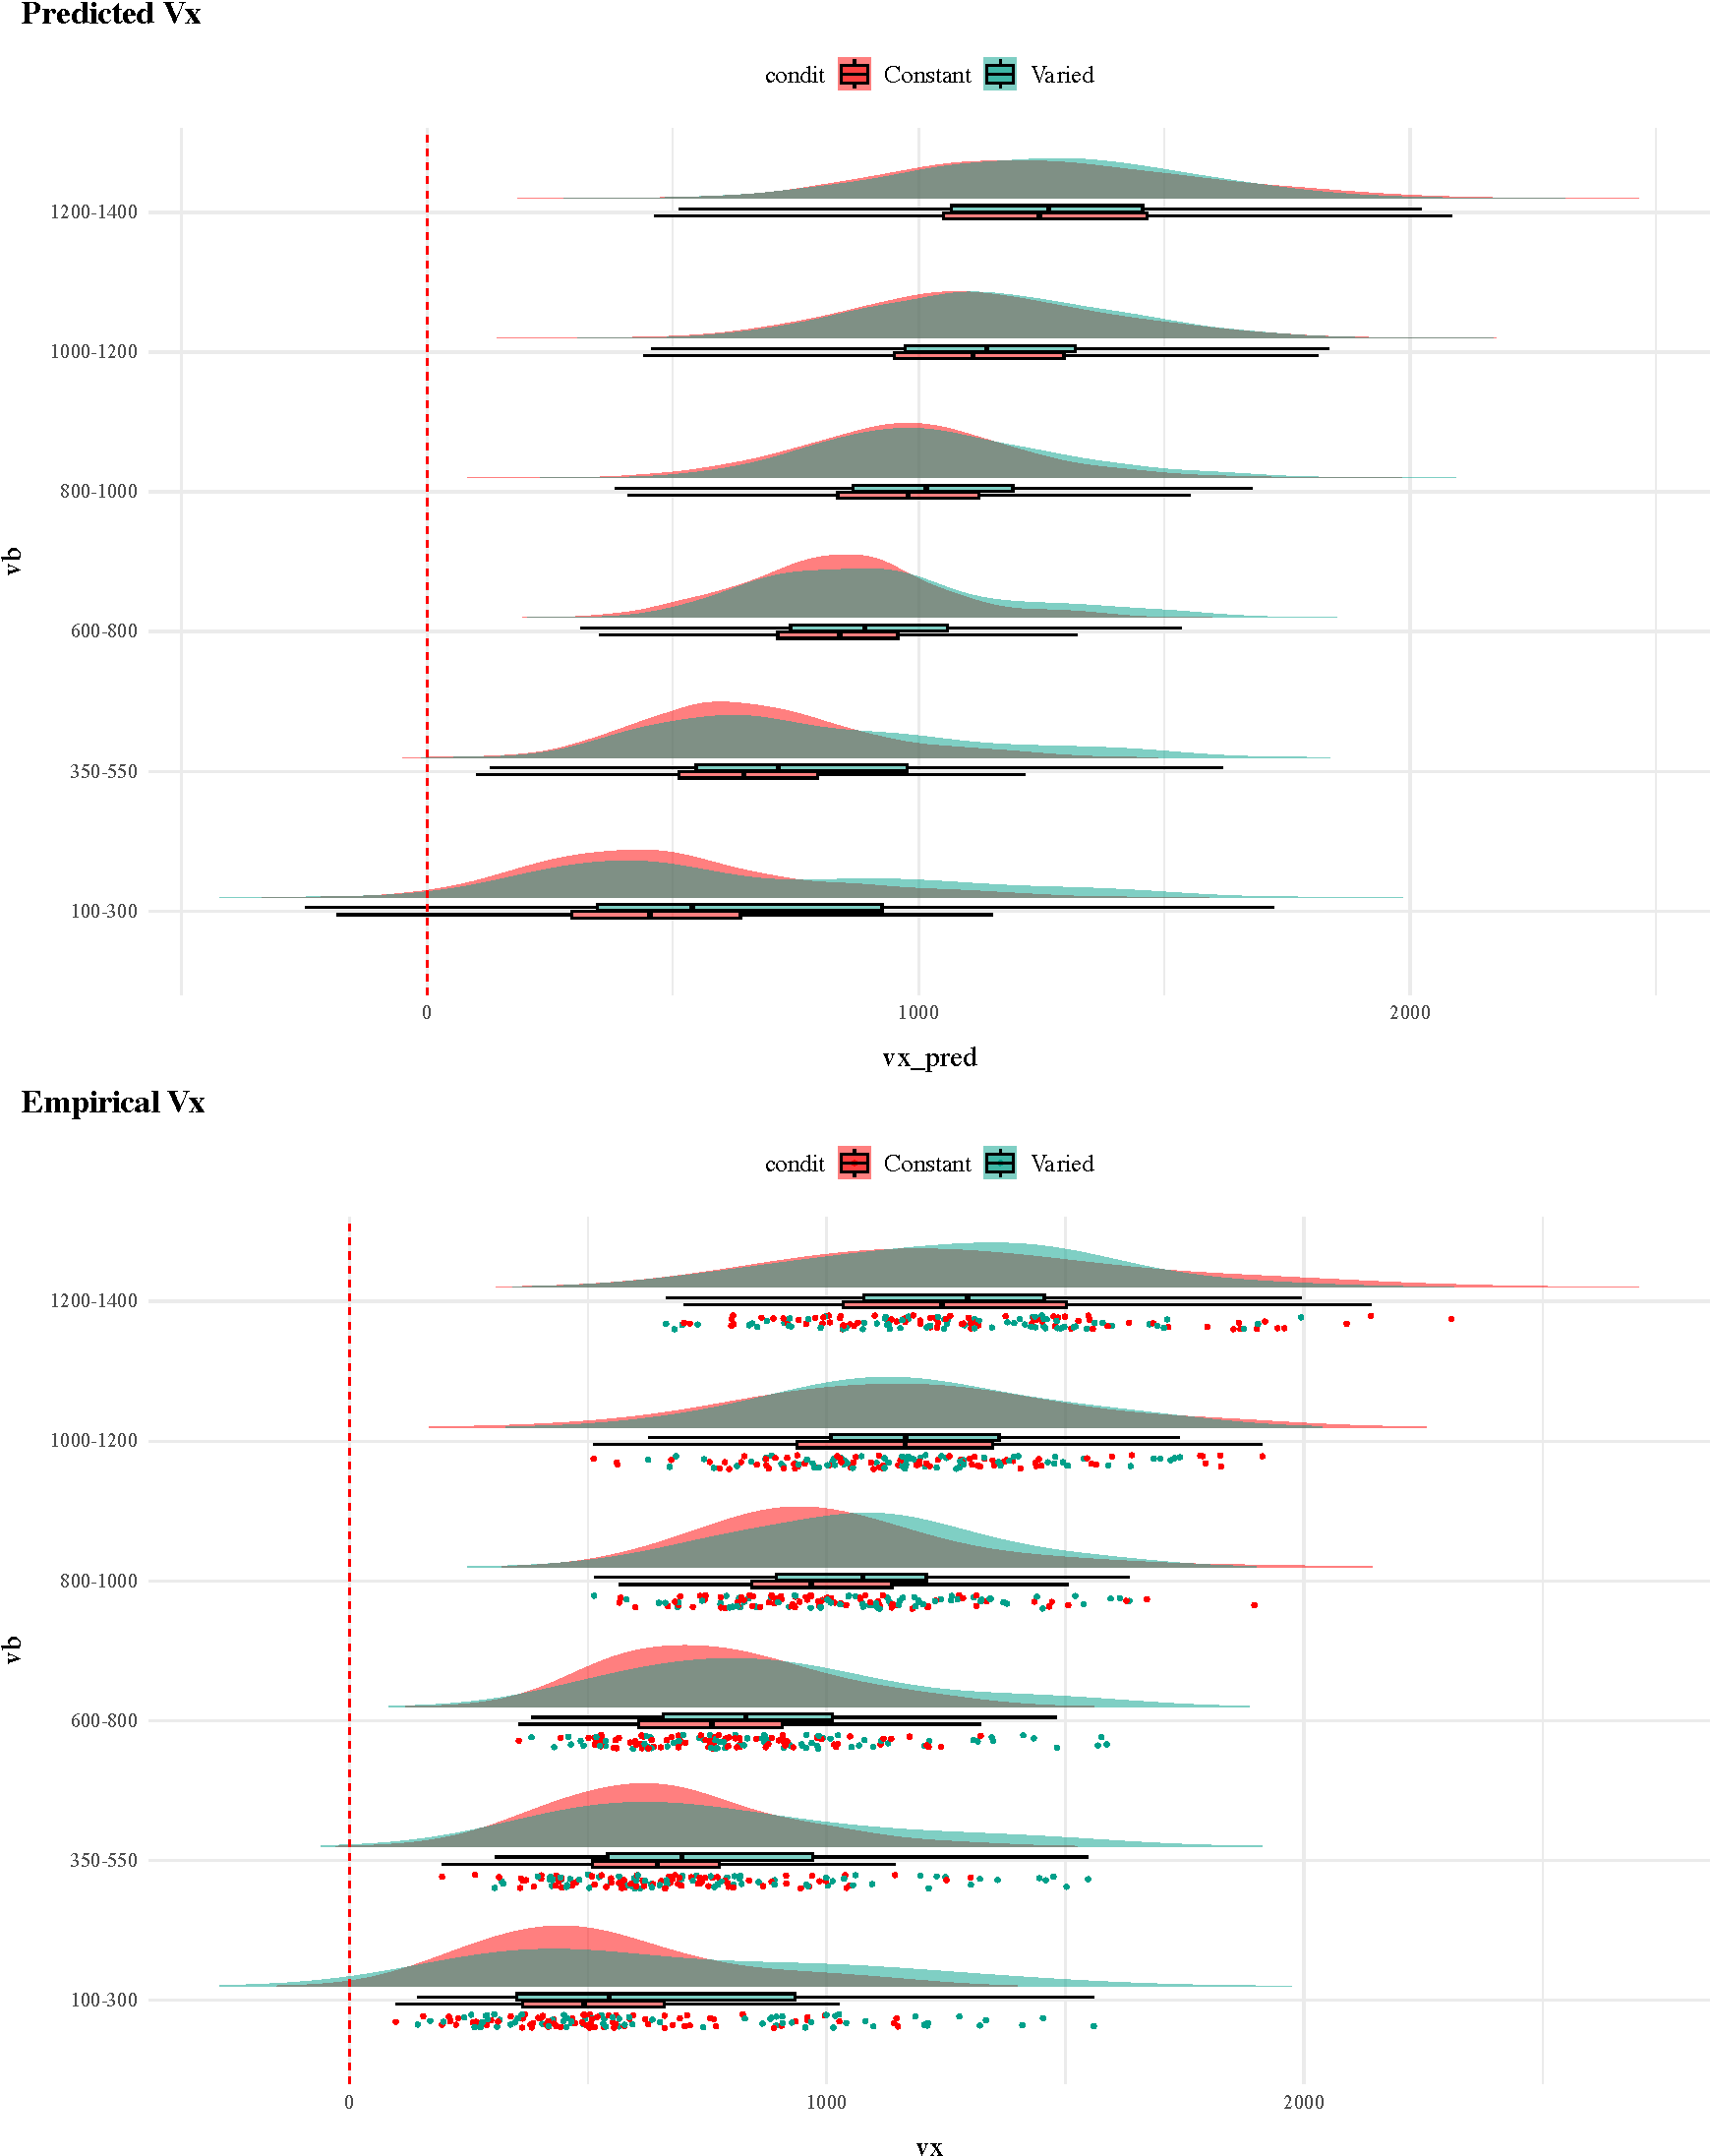
\includegraphics{igas_e1_files/figure-pdf/fig-empVsPred-1.pdf}

}

\caption{\label{fig-empVsPred}Bayesian Mixed Model predictions
vs.~Empirical Predictions - X velocity}

\end{figure}%

\paragraph{Different Aggregations}\label{different-aggregations}

\begin{Shaded}
\begin{Highlighting}[]
\NormalTok{epId }\OtherTok{\textless{}{-}}\NormalTok{ dist\_pred  }\SpecialCharTok{|\textgreater{}}
  \FunctionTok{filter}\NormalTok{(iter }\SpecialCharTok{\textless{}} \DecValTok{2}\NormalTok{)  }\SpecialCharTok{|\textgreater{}} \FunctionTok{group\_by}\NormalTok{(id,condit,vb) }\SpecialCharTok{|\textgreater{}}
  \FunctionTok{summarise}\NormalTok{(}\AttributeTok{dist=}\FunctionTok{median}\NormalTok{(dist)) }\SpecialCharTok{|\textgreater{}}
  \FunctionTok{ggplot}\NormalTok{(}\FunctionTok{aes}\NormalTok{(}\AttributeTok{x=}\NormalTok{vb,}\AttributeTok{y=}\NormalTok{dist,}\AttributeTok{fill=}\NormalTok{condit)) }\SpecialCharTok{+} 
  \FunctionTok{geom\_flat\_violin}\NormalTok{(}\FunctionTok{aes}\NormalTok{(}\AttributeTok{fill=}\NormalTok{condit), }\AttributeTok{position =} \FunctionTok{position\_nudge}\NormalTok{(}\AttributeTok{x =} \FloatTok{0.1}\NormalTok{, }\AttributeTok{y =} \DecValTok{0}\NormalTok{),}
                   \AttributeTok{adjust =} \FloatTok{1.5}\NormalTok{,}\AttributeTok{trim =} \ConstantTok{FALSE}\NormalTok{, }\AttributeTok{alpha =}\NormalTok{ .}\DecValTok{5}\NormalTok{, }\AttributeTok{colour =} \ConstantTok{NA}\NormalTok{) }\SpecialCharTok{+}
  \FunctionTok{geom\_point}\NormalTok{(}\FunctionTok{aes}\NormalTok{(}\AttributeTok{x =} \FunctionTok{as.numeric}\NormalTok{(vb) }\SpecialCharTok{{-}} \FloatTok{0.15}\NormalTok{, }\AttributeTok{col=}\NormalTok{condit),}
             \AttributeTok{position =} \FunctionTok{position\_jitter}\NormalTok{(}\AttributeTok{width =} \FloatTok{0.05}\NormalTok{, }\AttributeTok{height =} \DecValTok{0}\NormalTok{),}
             \AttributeTok{size =} \DecValTok{1}\NormalTok{, }\AttributeTok{shape =} \DecValTok{20}\NormalTok{, }\AttributeTok{alpha=}\NormalTok{.}\DecValTok{7}\NormalTok{) }\SpecialCharTok{+}
  \FunctionTok{geom\_boxplot}\NormalTok{(}\FunctionTok{aes}\NormalTok{(}\AttributeTok{x=}\NormalTok{vb,}\AttributeTok{y=}\NormalTok{dist,}\AttributeTok{fill=}\NormalTok{condit),}
               \AttributeTok{outlier.shape =} \ConstantTok{NA}\NormalTok{,}
               \AttributeTok{alpha =} \FloatTok{0.5}\NormalTok{, }\AttributeTok{width =} \FloatTok{0.1}\NormalTok{) }\SpecialCharTok{+}
  \FunctionTok{geom\_hline}\NormalTok{(}\AttributeTok{yintercept =} \DecValTok{0}\NormalTok{,}
             \AttributeTok{linetype =} \StringTok{\textquotesingle{}dashed\textquotesingle{}}\NormalTok{,}
             \AttributeTok{color =} \StringTok{\textquotesingle{}red\textquotesingle{}}\NormalTok{,}
             \AttributeTok{size =} \FloatTok{0.4}\NormalTok{) }\SpecialCharTok{+} 
  \FunctionTok{coord\_flip}\NormalTok{() }\SpecialCharTok{+} \FunctionTok{ggtitle}\NormalTok{(}\StringTok{"Empirical Deviation {-} Subject level averaging"}\NormalTok{) }



\NormalTok{epId }
\end{Highlighting}
\end{Shaded}

\begin{figure}[H]

\centering{

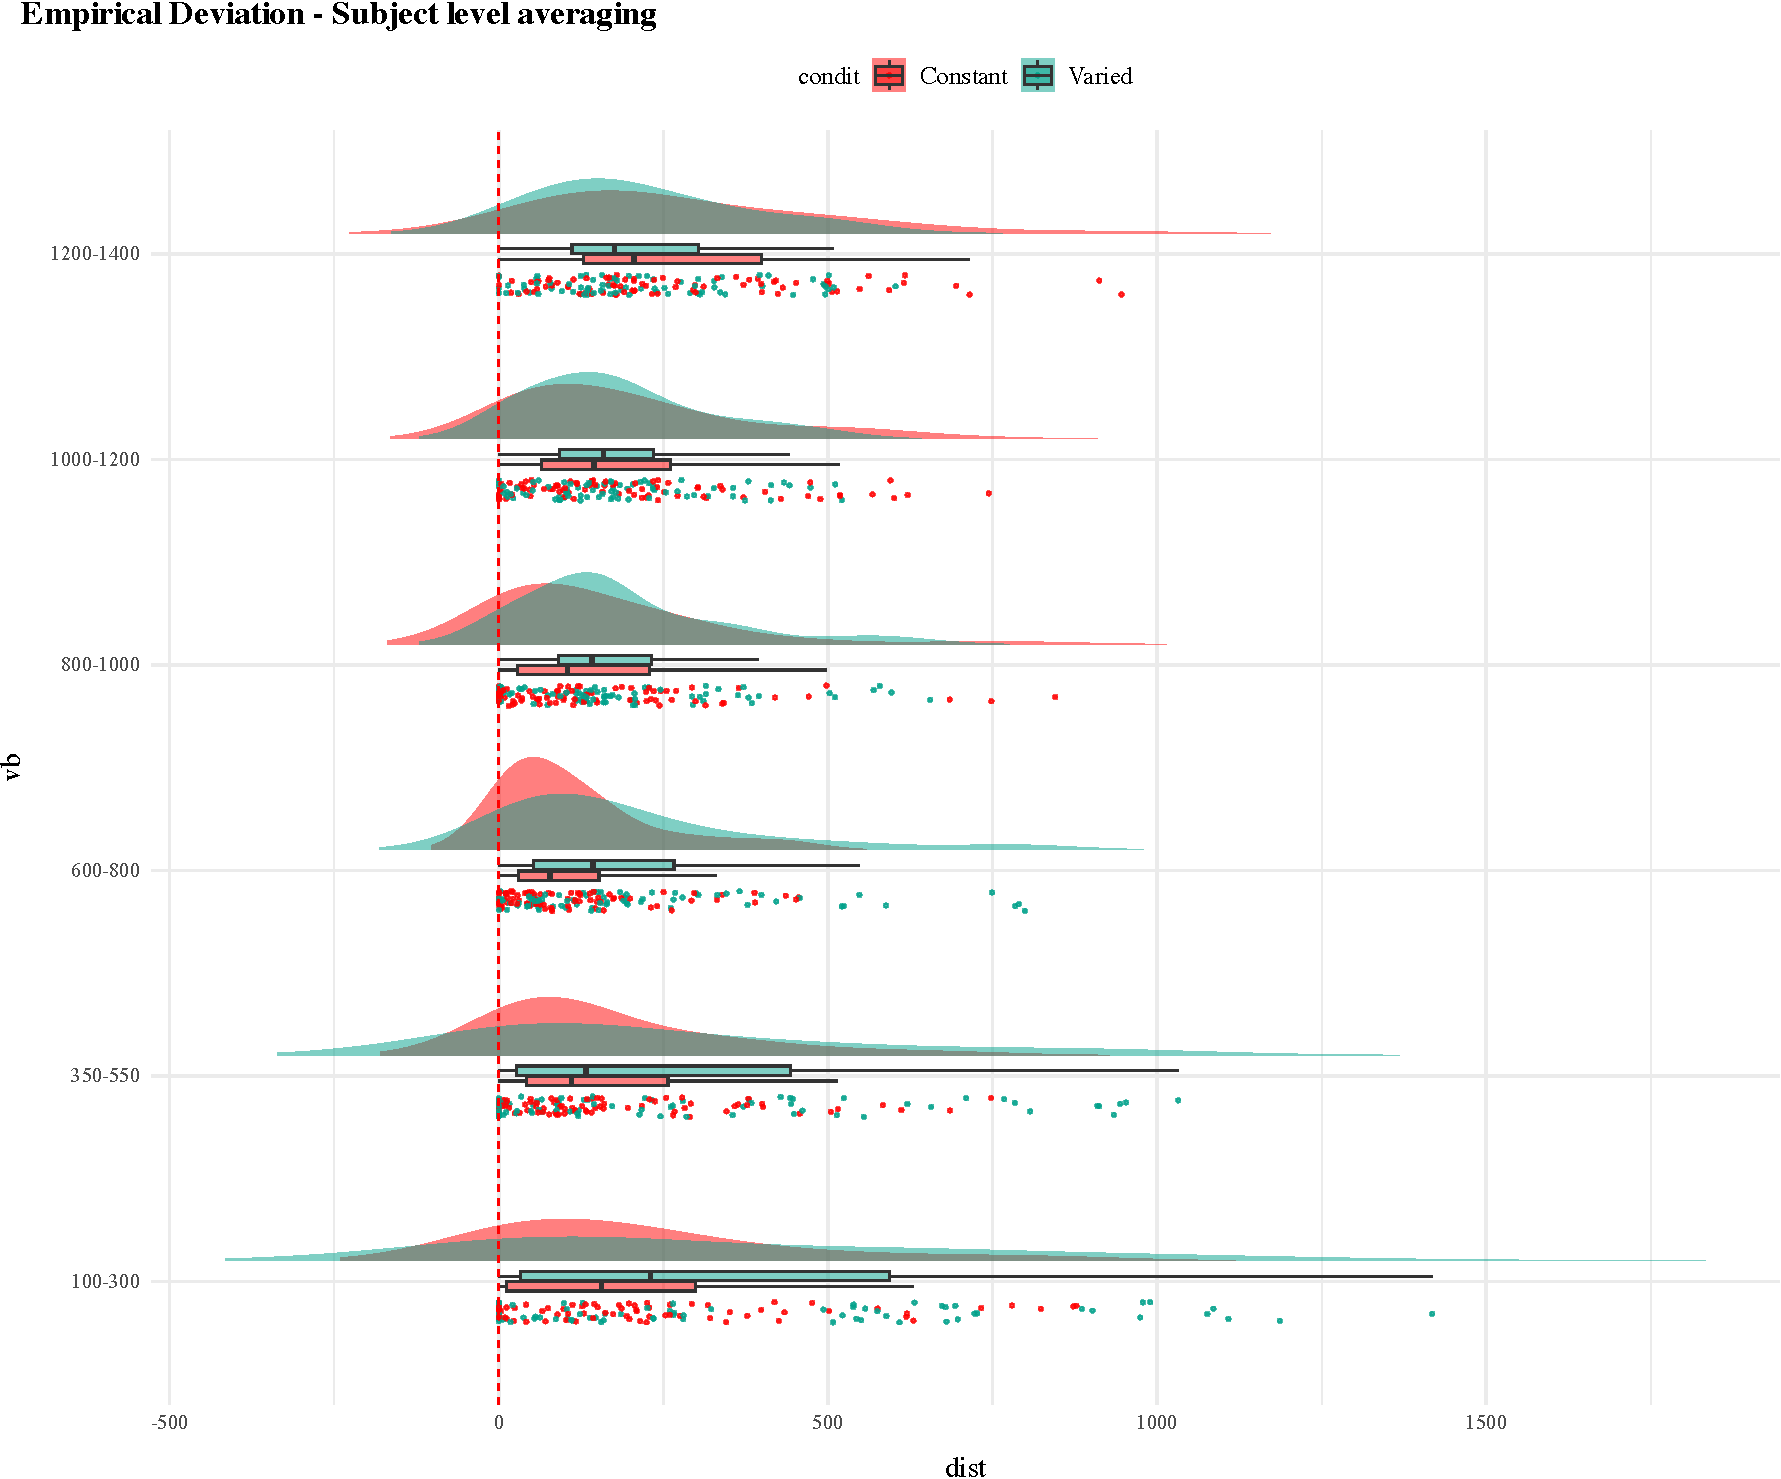
\includegraphics{igas_e1_files/figure-pdf/fig-empirical-distGrp1-1.pdf}

}

\caption{\label{fig-empirical-distGrp1}E1. Distribution of Vx at
Participant level}

\end{figure}%

\begin{Shaded}
\begin{Highlighting}[]
\NormalTok{epTrial }\OtherTok{\textless{}{-}}\NormalTok{ dist\_pred  }\SpecialCharTok{|\textgreater{}}
  \FunctionTok{filter}\NormalTok{(iter }\SpecialCharTok{\textless{}} \DecValTok{2}\NormalTok{)  }\SpecialCharTok{|\textgreater{}} \FunctionTok{group\_by}\NormalTok{(id,condit,vb) }\SpecialCharTok{|\textgreater{}}
  \FunctionTok{ggplot}\NormalTok{(}\FunctionTok{aes}\NormalTok{(}\AttributeTok{x=}\NormalTok{vb,}\AttributeTok{y=}\NormalTok{dist,}\AttributeTok{fill=}\NormalTok{condit)) }\SpecialCharTok{+} 
  \FunctionTok{geom\_flat\_violin}\NormalTok{(}\FunctionTok{aes}\NormalTok{(}\AttributeTok{fill=}\NormalTok{condit), }\AttributeTok{position =} \FunctionTok{position\_nudge}\NormalTok{(}\AttributeTok{x =} \FloatTok{0.1}\NormalTok{, }\AttributeTok{y =} \DecValTok{0}\NormalTok{),}
                   \AttributeTok{adjust =} \FloatTok{1.5}\NormalTok{,}\AttributeTok{trim =} \ConstantTok{FALSE}\NormalTok{, }\AttributeTok{alpha =}\NormalTok{ .}\DecValTok{5}\NormalTok{, }\AttributeTok{colour =} \ConstantTok{NA}\NormalTok{) }\SpecialCharTok{+}
  \FunctionTok{geom\_point}\NormalTok{(}\FunctionTok{aes}\NormalTok{(}\AttributeTok{x =} \FunctionTok{as.numeric}\NormalTok{(vb) }\SpecialCharTok{{-}} \FloatTok{0.15}\NormalTok{, }\AttributeTok{col=}\NormalTok{condit),}
             \AttributeTok{position =} \FunctionTok{position\_jitter}\NormalTok{(}\AttributeTok{width =} \FloatTok{0.05}\NormalTok{, }\AttributeTok{height =} \DecValTok{0}\NormalTok{),}
             \AttributeTok{size =}\NormalTok{ .}\DecValTok{5}\NormalTok{, }\AttributeTok{shape =} \DecValTok{20}\NormalTok{, }\AttributeTok{alpha=}\NormalTok{.}\DecValTok{7}\NormalTok{) }\SpecialCharTok{+}
  \FunctionTok{geom\_boxplot}\NormalTok{(}\FunctionTok{aes}\NormalTok{(}\AttributeTok{x=}\NormalTok{vb,}\AttributeTok{y=}\NormalTok{dist,}\AttributeTok{fill=}\NormalTok{condit),}
               \AttributeTok{outlier.shape =} \ConstantTok{NA}\NormalTok{,}
               \AttributeTok{alpha =} \FloatTok{0.5}\NormalTok{, }\AttributeTok{width =} \FloatTok{0.1}\NormalTok{) }\SpecialCharTok{+}
  \FunctionTok{geom\_hline}\NormalTok{(}\AttributeTok{yintercept =} \DecValTok{0}\NormalTok{,}
             \AttributeTok{linetype =} \StringTok{\textquotesingle{}dashed\textquotesingle{}}\NormalTok{,}
             \AttributeTok{color =} \StringTok{\textquotesingle{}red\textquotesingle{}}\NormalTok{,}
             \AttributeTok{size =} \FloatTok{0.4}\NormalTok{) }\SpecialCharTok{+} 
  \FunctionTok{coord\_flip}\NormalTok{() }\SpecialCharTok{+} \FunctionTok{ggtitle}\NormalTok{(}\StringTok{"Empirical Deviation {-} Raw Trial"}\NormalTok{) }\SpecialCharTok{+}
   \FunctionTok{theme}\NormalTok{(}\AttributeTok{axis.title.y=}\FunctionTok{element\_blank}\NormalTok{(),}
        \AttributeTok{axis.text.y=}\FunctionTok{element\_blank}\NormalTok{())}

\NormalTok{epTrial}
\end{Highlighting}
\end{Shaded}

\begin{figure}[H]

\centering{

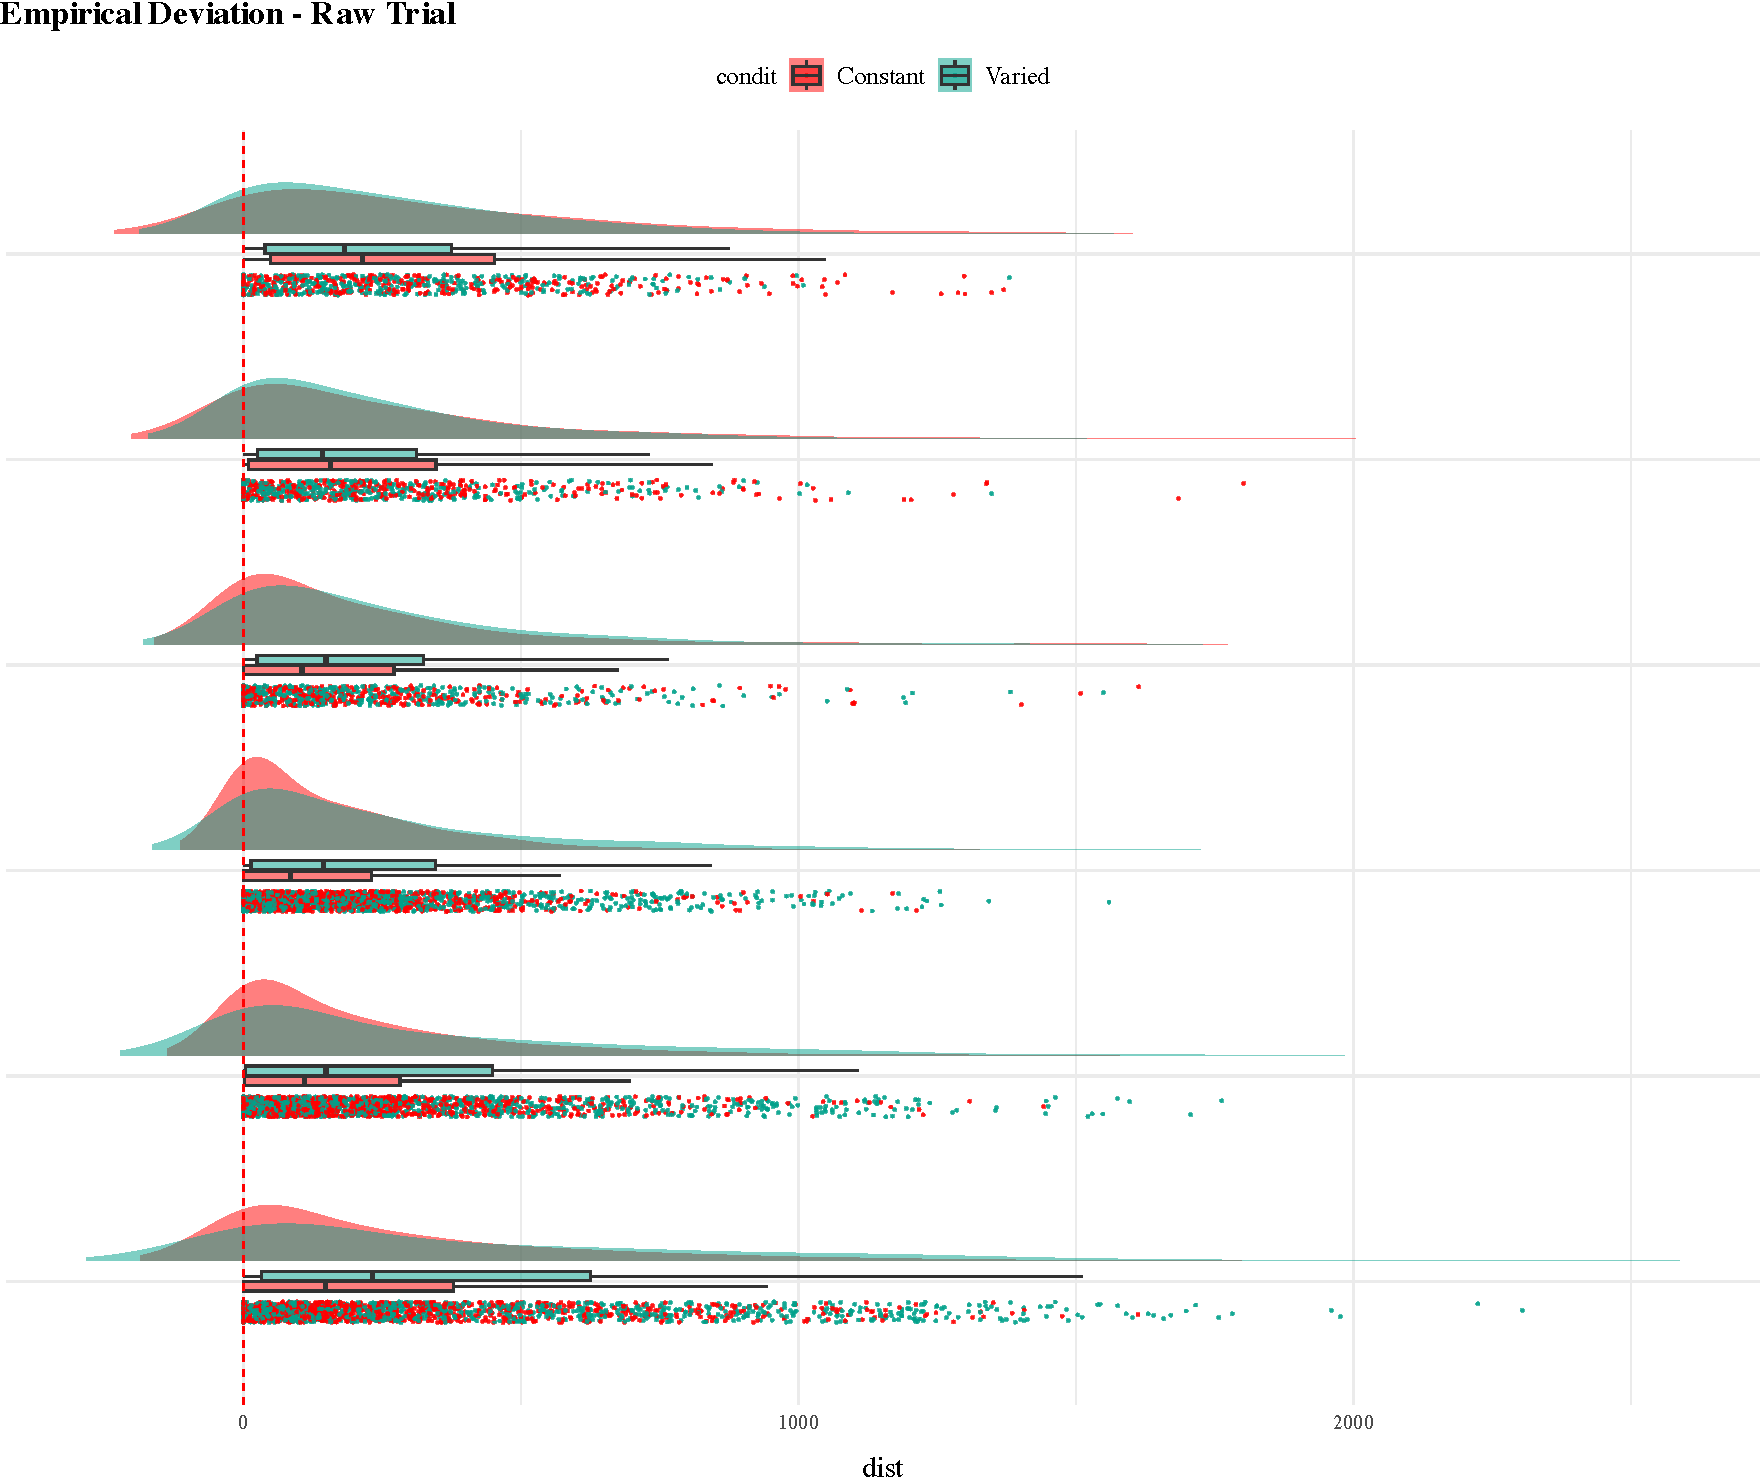
\includegraphics{igas_e1_files/figure-pdf/fig-empirical-distGrp2-1.pdf}

}

\caption{\label{fig-empirical-distGrp2}E1. Distribution of Vx at Trial
level}

\end{figure}%

\begin{Shaded}
\begin{Highlighting}[]
\NormalTok{new\_data\_grid}\OtherTok{=}\FunctionTok{map\_dfr}\NormalTok{(}\DecValTok{1}\NormalTok{, }\SpecialCharTok{\textasciitilde{}}\FunctionTok{data.frame}\NormalTok{(}\FunctionTok{unique}\NormalTok{(test[,}\FunctionTok{c}\NormalTok{(}\StringTok{"id"}\NormalTok{,}\StringTok{"condit"}\NormalTok{,}\StringTok{"bandInt"}\NormalTok{)])))}

\NormalTok{cSamp }\OtherTok{\textless{}{-}}\NormalTok{ e1\_distBMM  }\SpecialCharTok{|\textgreater{}} 
  \FunctionTok{emmeans}\NormalTok{(}\StringTok{"condit"}\NormalTok{,}\AttributeTok{by=}\StringTok{"bandInt"}\NormalTok{,}\AttributeTok{at=}\FunctionTok{list}\NormalTok{(}\AttributeTok{bandInt=}\FunctionTok{c}\NormalTok{(}\DecValTok{100}\NormalTok{,}\DecValTok{350}\NormalTok{,}\DecValTok{600}\NormalTok{,}\DecValTok{800}\NormalTok{,}\DecValTok{1000}\NormalTok{,}\DecValTok{1200}\NormalTok{)),}
          \AttributeTok{epred =} \ConstantTok{TRUE}\NormalTok{, }\AttributeTok{re\_formula =} \ConstantTok{NA}\NormalTok{) }\SpecialCharTok{|\textgreater{}} 
  \FunctionTok{pairs}\NormalTok{() }\SpecialCharTok{|\textgreater{}} \FunctionTok{gather\_emmeans\_draws}\NormalTok{()  }\SpecialCharTok{|\textgreater{}}
  \FunctionTok{group\_by}\NormalTok{(contrast, .draw,bandInt) }\SpecialCharTok{|\textgreater{}} \FunctionTok{summarise}\NormalTok{(}\AttributeTok{value=}\FunctionTok{mean}\NormalTok{(.value), }\AttributeTok{n=}\FunctionTok{n}\NormalTok{())}


\NormalTok{ ameBand }\OtherTok{\textless{}{-}}\NormalTok{ cSamp }\SpecialCharTok{|\textgreater{}} \FunctionTok{ggplot}\NormalTok{(}\FunctionTok{aes}\NormalTok{(}\AttributeTok{x=}\NormalTok{value,}\AttributeTok{y=}\StringTok{""}\NormalTok{)) }\SpecialCharTok{+} 
  \FunctionTok{stat\_halfeye}\NormalTok{() }\SpecialCharTok{+} 
  \FunctionTok{geom\_vline}\NormalTok{(}\AttributeTok{xintercept=}\DecValTok{0}\NormalTok{,}\AttributeTok{alpha=}\NormalTok{.}\DecValTok{4}\NormalTok{)}\SpecialCharTok{+}
  \FunctionTok{facet\_wrap}\NormalTok{(}\SpecialCharTok{\textasciitilde{}}\NormalTok{bandInt,}\AttributeTok{ncol=}\DecValTok{1}\NormalTok{) }\SpecialCharTok{+} \FunctionTok{labs}\NormalTok{(}\AttributeTok{x=}\StringTok{"Marginal Effect (Constant {-} Varied)"}\NormalTok{, }\AttributeTok{y=} \ConstantTok{NULL}\NormalTok{)}\SpecialCharTok{+}
  \FunctionTok{ggtitle}\NormalTok{(}\StringTok{"Average Marginal Effect"}\NormalTok{)}

\NormalTok{bothConditGM }\OtherTok{\textless{}{-}}\NormalTok{ e1\_distBMM }\SpecialCharTok{\%\textgreater{}\%}
  \FunctionTok{epred\_draws}\NormalTok{(}\AttributeTok{newdata =}\NormalTok{ new\_data\_grid,}\AttributeTok{ndraws =} \DecValTok{2000}\NormalTok{, }\AttributeTok{re\_formula =} \ConstantTok{NA}\NormalTok{) }\SpecialCharTok{|\textgreater{}}
  \FunctionTok{ggplot}\NormalTok{(}\FunctionTok{aes}\NormalTok{(}\AttributeTok{x=}\NormalTok{.epred,}\AttributeTok{y=}\StringTok{"Mean"}\NormalTok{,}\AttributeTok{fill=}\NormalTok{condit)) }\SpecialCharTok{+} 
  \FunctionTok{stat\_halfeye}\NormalTok{() }\SpecialCharTok{+}\FunctionTok{facet\_wrap}\NormalTok{(}\SpecialCharTok{\textasciitilde{}}\NormalTok{bandInt, }\AttributeTok{ncol =} \DecValTok{1}\NormalTok{) }\SpecialCharTok{+}
  \FunctionTok{labs}\NormalTok{(}\AttributeTok{x=}\StringTok{"Predicted Deviation"}\NormalTok{, }\AttributeTok{y=}\ConstantTok{NULL}\NormalTok{)}\SpecialCharTok{+}
  \FunctionTok{ggtitle}\NormalTok{(}\StringTok{"Grand Means"}\NormalTok{) }\SpecialCharTok{+}\FunctionTok{theme}\NormalTok{(}\AttributeTok{legend.position =} \StringTok{"bottom"}\NormalTok{)}

\NormalTok{(bothConditGM }\SpecialCharTok{|}\NormalTok{ ameBand) }\SpecialCharTok{+} \FunctionTok{plot\_layout}\NormalTok{(}\AttributeTok{widths=}\FunctionTok{c}\NormalTok{(}\DecValTok{2}\NormalTok{,}\FloatTok{1.0}\NormalTok{))}
\end{Highlighting}
\end{Shaded}

\begin{figure}[H]

\centering{

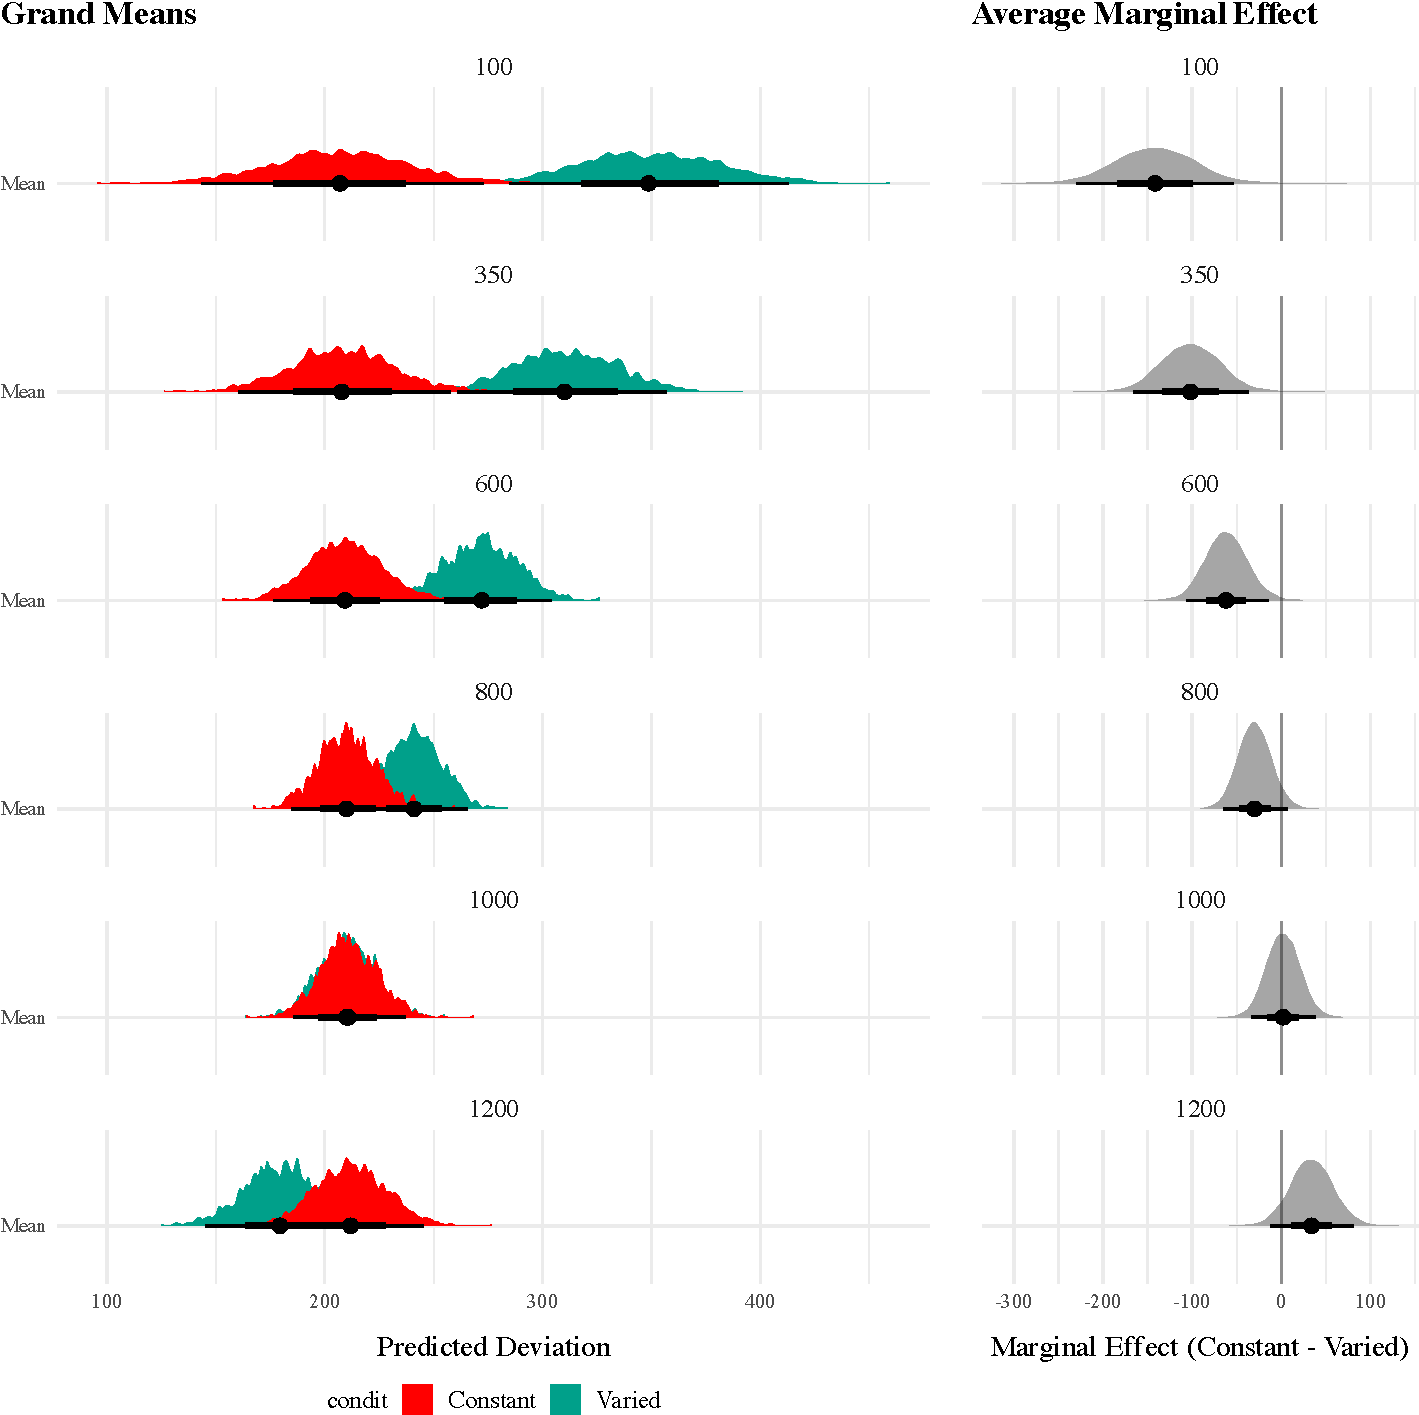
\includegraphics{igas_e1_files/figure-pdf/fig-e1-ame-1.pdf}

}

\caption{\label{fig-e1-ame}E1. Predicted Means Per Condition and Band,
and Average Marginal Effect (Constant - Varied)}

\end{figure}%

\section*{References}\label{references}
\addcontentsline{toc}{section}{References}

\phantomsection\label{refs}
\begin{CSLReferences}{1}{0}
\bibitem[\citeproctext]{ref-deloshExtrapolationSineQua1997}
DeLosh, E. L., McDaniel, M. A., \& Busemeyer, J. R. (1997).
Extrapolation: {The Sine Qua Non} for {Abstraction} in {Function
Learning}. \emph{Journal of Experimental Psychology: Learning, Memory,
and Cognition}, \emph{23}(4), 19.
\url{https://doi.org/10.1037/0278-7393.23.4.968}

\bibitem[\citeproctext]{ref-mcdanielPredictingTransferPerformance2009}
Mcdaniel, M. A., Dimperio, E., Griego, J. A., \& Busemeyer, J. R.
(2009). Predicting transfer performance: {A} comparison of competing
function learning models. \emph{Journal of Experimental Psychology.
Learning, Memory, and Cognition}, \emph{35}, 173--195.
\url{https://doi.org/10.1037/a0013982}

\end{CSLReferences}



\end{document}
